% Options for packages loaded elsewhere
\PassOptionsToPackage{unicode}{hyperref}
\PassOptionsToPackage{hyphens}{url}
%
\documentclass[
  man,floatsintext]{apa6}
\usepackage{amsmath,amssymb}
\usepackage{iftex}
\ifPDFTeX
  \usepackage[T1]{fontenc}
  \usepackage[utf8]{inputenc}
  \usepackage{textcomp} % provide euro and other symbols
\else % if luatex or xetex
  \usepackage{unicode-math} % this also loads fontspec
  \defaultfontfeatures{Scale=MatchLowercase}
  \defaultfontfeatures[\rmfamily]{Ligatures=TeX,Scale=1}
\fi
\usepackage{lmodern}
\ifPDFTeX\else
  % xetex/luatex font selection
\fi
% Use upquote if available, for straight quotes in verbatim environments
\IfFileExists{upquote.sty}{\usepackage{upquote}}{}
\IfFileExists{microtype.sty}{% use microtype if available
  \usepackage[]{microtype}
  \UseMicrotypeSet[protrusion]{basicmath} % disable protrusion for tt fonts
}{}
\makeatletter
\@ifundefined{KOMAClassName}{% if non-KOMA class
  \IfFileExists{parskip.sty}{%
    \usepackage{parskip}
  }{% else
    \setlength{\parindent}{0pt}
    \setlength{\parskip}{6pt plus 2pt minus 1pt}}
}{% if KOMA class
  \KOMAoptions{parskip=half}}
\makeatother
\usepackage{xcolor}
\usepackage{color}
\usepackage{fancyvrb}
\newcommand{\VerbBar}{|}
\newcommand{\VERB}{\Verb[commandchars=\\\{\}]}
\DefineVerbatimEnvironment{Highlighting}{Verbatim}{commandchars=\\\{\}}
% Add ',fontsize=\small' for more characters per line
\usepackage{framed}
\definecolor{shadecolor}{RGB}{248,248,248}
\newenvironment{Shaded}{\begin{snugshade}}{\end{snugshade}}
\newcommand{\AlertTok}[1]{\textcolor[rgb]{0.94,0.16,0.16}{#1}}
\newcommand{\AnnotationTok}[1]{\textcolor[rgb]{0.56,0.35,0.01}{\textbf{\textit{#1}}}}
\newcommand{\AttributeTok}[1]{\textcolor[rgb]{0.13,0.29,0.53}{#1}}
\newcommand{\BaseNTok}[1]{\textcolor[rgb]{0.00,0.00,0.81}{#1}}
\newcommand{\BuiltInTok}[1]{#1}
\newcommand{\CharTok}[1]{\textcolor[rgb]{0.31,0.60,0.02}{#1}}
\newcommand{\CommentTok}[1]{\textcolor[rgb]{0.56,0.35,0.01}{\textit{#1}}}
\newcommand{\CommentVarTok}[1]{\textcolor[rgb]{0.56,0.35,0.01}{\textbf{\textit{#1}}}}
\newcommand{\ConstantTok}[1]{\textcolor[rgb]{0.56,0.35,0.01}{#1}}
\newcommand{\ControlFlowTok}[1]{\textcolor[rgb]{0.13,0.29,0.53}{\textbf{#1}}}
\newcommand{\DataTypeTok}[1]{\textcolor[rgb]{0.13,0.29,0.53}{#1}}
\newcommand{\DecValTok}[1]{\textcolor[rgb]{0.00,0.00,0.81}{#1}}
\newcommand{\DocumentationTok}[1]{\textcolor[rgb]{0.56,0.35,0.01}{\textbf{\textit{#1}}}}
\newcommand{\ErrorTok}[1]{\textcolor[rgb]{0.64,0.00,0.00}{\textbf{#1}}}
\newcommand{\ExtensionTok}[1]{#1}
\newcommand{\FloatTok}[1]{\textcolor[rgb]{0.00,0.00,0.81}{#1}}
\newcommand{\FunctionTok}[1]{\textcolor[rgb]{0.13,0.29,0.53}{\textbf{#1}}}
\newcommand{\ImportTok}[1]{#1}
\newcommand{\InformationTok}[1]{\textcolor[rgb]{0.56,0.35,0.01}{\textbf{\textit{#1}}}}
\newcommand{\KeywordTok}[1]{\textcolor[rgb]{0.13,0.29,0.53}{\textbf{#1}}}
\newcommand{\NormalTok}[1]{#1}
\newcommand{\OperatorTok}[1]{\textcolor[rgb]{0.81,0.36,0.00}{\textbf{#1}}}
\newcommand{\OtherTok}[1]{\textcolor[rgb]{0.56,0.35,0.01}{#1}}
\newcommand{\PreprocessorTok}[1]{\textcolor[rgb]{0.56,0.35,0.01}{\textit{#1}}}
\newcommand{\RegionMarkerTok}[1]{#1}
\newcommand{\SpecialCharTok}[1]{\textcolor[rgb]{0.81,0.36,0.00}{\textbf{#1}}}
\newcommand{\SpecialStringTok}[1]{\textcolor[rgb]{0.31,0.60,0.02}{#1}}
\newcommand{\StringTok}[1]{\textcolor[rgb]{0.31,0.60,0.02}{#1}}
\newcommand{\VariableTok}[1]{\textcolor[rgb]{0.00,0.00,0.00}{#1}}
\newcommand{\VerbatimStringTok}[1]{\textcolor[rgb]{0.31,0.60,0.02}{#1}}
\newcommand{\WarningTok}[1]{\textcolor[rgb]{0.56,0.35,0.01}{\textbf{\textit{#1}}}}
\usepackage{graphicx}
\makeatletter
\def\maxwidth{\ifdim\Gin@nat@width>\linewidth\linewidth\else\Gin@nat@width\fi}
\def\maxheight{\ifdim\Gin@nat@height>\textheight\textheight\else\Gin@nat@height\fi}
\makeatother
% Scale images if necessary, so that they will not overflow the page
% margins by default, and it is still possible to overwrite the defaults
% using explicit options in \includegraphics[width, height, ...]{}
\setkeys{Gin}{width=\maxwidth,height=\maxheight,keepaspectratio}
% Set default figure placement to htbp
\makeatletter
\def\fps@figure{htbp}
\makeatother
\setlength{\emergencystretch}{3em} % prevent overfull lines
\providecommand{\tightlist}{%
  \setlength{\itemsep}{0pt}\setlength{\parskip}{0pt}}
\setcounter{secnumdepth}{-\maxdimen} % remove section numbering
% Make \paragraph and \subparagraph free-standing
\ifx\paragraph\undefined\else
  \let\oldparagraph\paragraph
  \renewcommand{\paragraph}[1]{\oldparagraph{#1}\mbox{}}
\fi
\ifx\subparagraph\undefined\else
  \let\oldsubparagraph\subparagraph
  \renewcommand{\subparagraph}[1]{\oldsubparagraph{#1}\mbox{}}
\fi
% definitions for citeproc citations
\NewDocumentCommand\citeproctext{}{}
\NewDocumentCommand\citeproc{mm}{%
  \begingroup\def\citeproctext{#2}\cite{#1}\endgroup}
\makeatletter
 % allow citations to break across lines
 \let\@cite@ofmt\@firstofone
 % avoid brackets around text for \cite:
 \def\@biblabel#1{}
 \def\@cite#1#2{{#1\if@tempswa , #2\fi}}
\makeatother
\newlength{\cslhangindent}
\setlength{\cslhangindent}{1.5em}
\newlength{\csllabelwidth}
\setlength{\csllabelwidth}{3em}
\newenvironment{CSLReferences}[2] % #1 hanging-indent, #2 entry-spacing
 {\begin{list}{}{%
  \setlength{\itemindent}{0pt}
  \setlength{\leftmargin}{0pt}
  \setlength{\parsep}{0pt}
  % turn on hanging indent if param 1 is 1
  \ifodd #1
   \setlength{\leftmargin}{\cslhangindent}
   \setlength{\itemindent}{-1\cslhangindent}
  \fi
  % set entry spacing
  \setlength{\itemsep}{#2\baselineskip}}}
 {\end{list}}
\usepackage{calc}
\newcommand{\CSLBlock}[1]{\hfill\break\parbox[t]{\linewidth}{\strut\ignorespaces#1\strut}}
\newcommand{\CSLLeftMargin}[1]{\parbox[t]{\csllabelwidth}{\strut#1\strut}}
\newcommand{\CSLRightInline}[1]{\parbox[t]{\linewidth - \csllabelwidth}{\strut#1\strut}}
\newcommand{\CSLIndent}[1]{\hspace{\cslhangindent}#1}
\ifLuaTeX
\usepackage[bidi=basic]{babel}
\else
\usepackage[bidi=default]{babel}
\fi
\babelprovide[main,import]{english}
% get rid of language-specific shorthands (see #6817):
\let\LanguageShortHands\languageshorthands
\def\languageshorthands#1{}
% Manuscript styling
\usepackage{upgreek}
\captionsetup{font=singlespacing,justification=justified}

% Table formatting
\usepackage{longtable}
\usepackage{lscape}
% \usepackage[counterclockwise]{rotating}   % Landscape page setup for large tables
\usepackage{multirow}		% Table styling
\usepackage{tabularx}		% Control Column width
\usepackage[flushleft]{threeparttable}	% Allows for three part tables with a specified notes section
\usepackage{threeparttablex}            % Lets threeparttable work with longtable

% Create new environments so endfloat can handle them
% \newenvironment{ltable}
%   {\begin{landscape}\centering\begin{threeparttable}}
%   {\end{threeparttable}\end{landscape}}
\newenvironment{lltable}{\begin{landscape}\centering\begin{ThreePartTable}}{\end{ThreePartTable}\end{landscape}}

% Enables adjusting longtable caption width to table width
% Solution found at http://golatex.de/longtable-mit-caption-so-breit-wie-die-tabelle-t15767.html
\makeatletter
\newcommand\LastLTentrywidth{1em}
\newlength\longtablewidth
\setlength{\longtablewidth}{1in}
\newcommand{\getlongtablewidth}{\begingroup \ifcsname LT@\roman{LT@tables}\endcsname \global\longtablewidth=0pt \renewcommand{\LT@entry}[2]{\global\advance\longtablewidth by ##2\relax\gdef\LastLTentrywidth{##2}}\@nameuse{LT@\roman{LT@tables}} \fi \endgroup}

% \setlength{\parindent}{0.5in}
% \setlength{\parskip}{0pt plus 0pt minus 0pt}

% Overwrite redefinition of paragraph and subparagraph by the default LaTeX template
% See https://github.com/crsh/papaja/issues/292
\makeatletter
\renewcommand{\paragraph}{\@startsection{paragraph}{4}{\parindent}%
  {0\baselineskip \@plus 0.2ex \@minus 0.2ex}%
  {-1em}%
  {\normalfont\normalsize\bfseries\itshape\typesectitle}}

\renewcommand{\subparagraph}[1]{\@startsection{subparagraph}{5}{1em}%
  {0\baselineskip \@plus 0.2ex \@minus 0.2ex}%
  {-\z@\relax}%
  {\normalfont\normalsize\itshape\hspace{\parindent}{#1}\textit{\addperi}}{\relax}}
\makeatother

% \usepackage{etoolbox}
\makeatletter
\patchcmd{\HyOrg@maketitle}
  {\section{\normalfont\normalsize\abstractname}}
  {\section*{\normalfont\normalsize\abstractname}}
  {}{\typeout{Failed to patch abstract.}}
\patchcmd{\HyOrg@maketitle}
  {\section{\protect\normalfont{\@title}}}
  {\section*{\protect\normalfont{\@title}}}
  {}{\typeout{Failed to patch title.}}
\makeatother

\usepackage{xpatch}
\makeatletter
\xapptocmd\appendix
  {\xapptocmd\section
    {\addcontentsline{toc}{section}{\appendixname\ifoneappendix\else~\theappendix\fi\\: #1}}
    {}{\InnerPatchFailed}%
  }
{}{\PatchFailed}
\keywords{\newline\indent Word count: 4819}
\usepackage{csquotes}
\ifLuaTeX
  \usepackage{selnolig}  % disable illegal ligatures
\fi
\IfFileExists{bookmark.sty}{\usepackage{bookmark}}{\usepackage{hyperref}}
\IfFileExists{xurl.sty}{\usepackage{xurl}}{} % add URL line breaks if available
\urlstyle{same}
\hypersetup{
  pdftitle={Unveiling Echo Chambers on YouTube: Analyzing Political Discourse and Social Dynamics Through Advanced Quantitative Methods},
  pdfauthor={Roman Nekrasov, Huub van de Voort, Andy Huang, Oumaima Lemhour, \& Tom Teurlings},
  pdflang={en-EN},
  hidelinks,
  pdfcreator={LaTeX via pandoc}}

\title{Unveiling Echo Chambers on YouTube: Analyzing Political Discourse and Social Dynamics Through Advanced Quantitative Methods}
\author{Roman Nekrasov\textsuperscript{}, Huub van de Voort\textsuperscript{}, Andy Huang\textsuperscript{}, Oumaima Lemhour\textsuperscript{}, \& Tom Teurlings\textsuperscript{}}
\date{December 2023}


\shorttitle{YouTube Echo Chambers}

\affiliation{\vspace{0.5cm}\textsuperscript{} Jheronimus Academy of Data Science}

\begin{document}
\maketitle

\section*{Executive Summary}\label{executive-summary}
\addcontentsline{toc}{section}{Executive Summary}

This study explores the phenomenon of echo chambers on YouTube. It aims to understand how certain users or groups influence conversations and network structures, particularly in the context of politically charged content on smaller, politically focused YouTube channels. The study employs advanced quantitative methods, including Exponential Random Graph Models (ERGMs) and centrality measures, to analyze the presence and impact of prominent users in YouTube comment sections and the existence of echo chambers within these sections. The results contribute to a deeper understanding of social interactions on YouTube, addressing gaps and offering new insights into the platform's social dynamics, especially related to far-right content.

\section{Introduction}\label{introduction}

Research on social media platforms, such as Twitter and Facebook, extensively explores echo chambers - environments where individuals connect with like-minded peers, reinforcing selective exposure to information aligning with their beliefs (Cinelli, De Francisci Morales, Galeazzi, Quattrociocchi, \& Starnini, 2021). These principles, observed on social media platforms marked by informational homogeneity, apply to broader political discourse and policy debates (Jasny, Waggle, \& Fisher, 2015). This suggests that the mechanisms of selective exposure observed in social media echo chambers may extend to diverse communication networks (Colleoni, Rozza, \& Arvidsson, 2014). These tendencies contribute to polarization and extreme political positions (Colleoni et al., 2014). This harms social cohesion and trust, challenging finding common ground between political parties (McCoy \& Somer, 2019) and shaping public discourse across diverse communication networks (Levy \& Razin, 2019). Despite extensive research on platforms such as Twitter, the impact of echo chambers on YouTube, the second-largest social platform, remains understudied. YouTube's unique structure and user interaction patterns, distinct from platforms like Twitter, may pose challenges in recognizing and understanding echo chambers on this platform.
Recent research in social network analysis indicates a weaker presence of echo chambers, showing a tendency towards heterogeneity in discussions, even on controversial topics (Röchert, Neubaum, Ross, Brachten, \& Stieglitz, 2020). However, prior research aggregates comment threads from numerous videos or focuses on singular, high-traffic videos, potentially overlooking the enclosed homogenous interactions typical of echo chambers. This methodological limitation risks underestimating their presence and influence on YouTube. Evidence from Hosseinmardi et al.~(2020) challenges assumptions about algorithmic amplification in YouTube echo chambers, revealing them to be more subtle and insular than previously understood (Hosseinmardi et al., 2020). With the recent addition of user handles on YouTube, allowing individuals to tag each other, there has been a shift in user interactions (YouTube, 2022). This new feature holds the potential to offer insights into the formation of echo chambers, an aspect earlier research did not investigate. The identified gaps, coupled with recent changes in user interactions, necessitate a more targeted approach to precisely capture and analyze the evolving dynamics of social networks, revealing how echo chambers form and influence discourse.
The concern about echo chamber effects in online communities, especially on social media platforms, is pronounced. Research by Cinelli (2021) and Du et al.~(2017) emphasizes the contribution of echo chambers to heightened polarization and the formation of distinct opposing groups with online communities (Cinelli et al., 2021; Du \& Gregory, 2017). Platforms like Twitter exemplify polarization attributed to echo chamber effects (Du \& Gregory, 2017). This trend is alarming as social media platforms evolve from sources of entertainment to influential shapers of the social narrative. Echo chamber effects impact critical aspects of society, including policy-making, political communication and public discourse on controversial subjects (Cinelli et al., 2021). Grusauskaite, Carbone, Harambam, and Aupers (2023) underlines this concern, emphasizing social media's role in deepening societal divides and fueling extremist ideologies (Grusauskaite et al., 2023). This highlights the importance of investigating echo chamber contexts on YouTube. The heightened significance arises from individuals perceiving videos as more credible than text, particularly in politics (Wittenberg, Tappin, Berinsky, \& Rand, 2021). Given YouTube's status as the largest and most engaging online media consumption platform globally (Hosseinmardi et al., 2020), there is a pressing need to investigate echo chambers within its channels.
To investigate YouTube echo chambers, our study proposes examining smaller, politically focused videos or channels with pronounced viewpoints. This approach aligns with research indicating a higher likelihood of echo chambers in political discussions (Villa, Pasi, \& Viviani, 2021). Our focus on potentially more insular communities aims to uncover the true extent and nature of echo chambers on YouTube, contributing a nuanced understanding of the platform's social dynamics, especially related to far-right content (Hosseinmardi et al., 2020).

This will be done by conducting two studies:

\textbf{RQ 1 } \emph{To what extent are prominent users present within YouTube channels' comment sections?}
This study explores the presence of prominent users within YouTube channels' comment networks and their impact on the network structure. We hypothesize that YouTube comment sections feature influential users, drawing a parallel to the social network dynamics observed on Twitter (Sung, Moon, \& Lee, 2013). This is based on the observed similarities in the structural dynamics of these platforms' social networks (Wattenhofer, Wattenhofer, \& Zhu, 2012). We will use centrality measures to evaluate the extent of prominent users' presence in YouTube comment sections. These measures will provide quantitative insights into the influence and connectivity of users within the network. Conditional uniform graphs (CUGs) will be used to contextualize and validate these findings. CUGs will enable us to determine whether the centrality measures observed in the YouTube comment networks are exceptionally high or low, compared to what might be expected in a randomly structured network.

\textbf{RQ 2} \emph{To what extent are there echo chambers within YouTube channels’ comment sections?}
The second study explores the existence of echo chambers within the comment sections of YouTube channels. Building upon our earlier research, which we discussed before, we hypothesize that echo chambers will be present in YouTube channels' comment sections which have a politically pronounced viewpoint. We use Exponential Random Graph Models (ERGMs) to test this hypothesis. This statistical framework allows us to examine the structural patterns of relationships in YouTube comments, providing insights into echo chambers' emergence and characteristics within these channels.
By answering these research questions, our study contributes to understanding social interactions on YouTube, addressing gaps and exploring new dimensions. These insights are important to grasp how certain individuals or groups can influence conversations and network structures. Our second study investigates the presence and nature of echo chambers, thereby addressing concerns about social media's role in promoting ideological division and polarization. These findings will enhance our understanding of how certain users can initiate or reinforce echo chamber dynamics, leading to a more homogenous environment where similar viewpoints are echoed and amplified. Consequently, these individuals and dynamics can increase polarization and reduce exposure to diverse perspectives, affecting public discourse and social cohesion.
In the remainder of the report, we will progress from discussing the dataset to outlining the rationale behind our chosen research methods. We then present and discuss the results of our studies and conclude with a summary of our findings, their implications and suggestions for future research. ~

\newpage

\section{Methodology}\label{methodology}

\subsection{Dataset}\label{dataset}

A dataset was assembled by scraping the YouTube comment section. Ongehoord Nederland was selected for its unique nature as a YouTube channel, as it is known for broadcasting controversial and pronounced right-wing-oriented viewpoints. Having also compared Ongehoord Nederland to other right-wing-oriented channels in terms of channel subscribers, views and videos it is relatively a small channel. Together, this makes it an appropriate channel for our study's focus on political echo chambers, especially considering the channel's scale and content nature, which align with the methodological pivot outlined earlier.
The larger the dataset, the more computationally expensive it is. Hence, we randomly selected a sequence of five videos from the channel. Rather than choosing videos randomly across the channel's history, this approach was intended to increase the chances of finding users who commented on
multiple videos. Selecting sequentially adjacent videos, yet chosen randomly, allows for a more integrated analysis of user interactions and patterns, avoiding the disjointedness that might arise from sampling videos from widely separated time periods on the channel.
In our dataset, nodes correspond to YouTube users engaged in the comment section using handles, which are unique and short identifiers and start with the ``@'' symbol. Directed edges in our network are formed based on explicit user interactions. This occurs when a user directly references another by their handle in a comment or is similarly mentioned by others. We restrict our analysis to interactions involving handles, as this clearly indicates directed communication. Comments without such specific mentions are excluded, as we cannot conclusively determine if they are responses to the main thread or to specific individuals, thus ensuring clarity and precision in our network analysis.



\begin{figure}[H]

{\centering 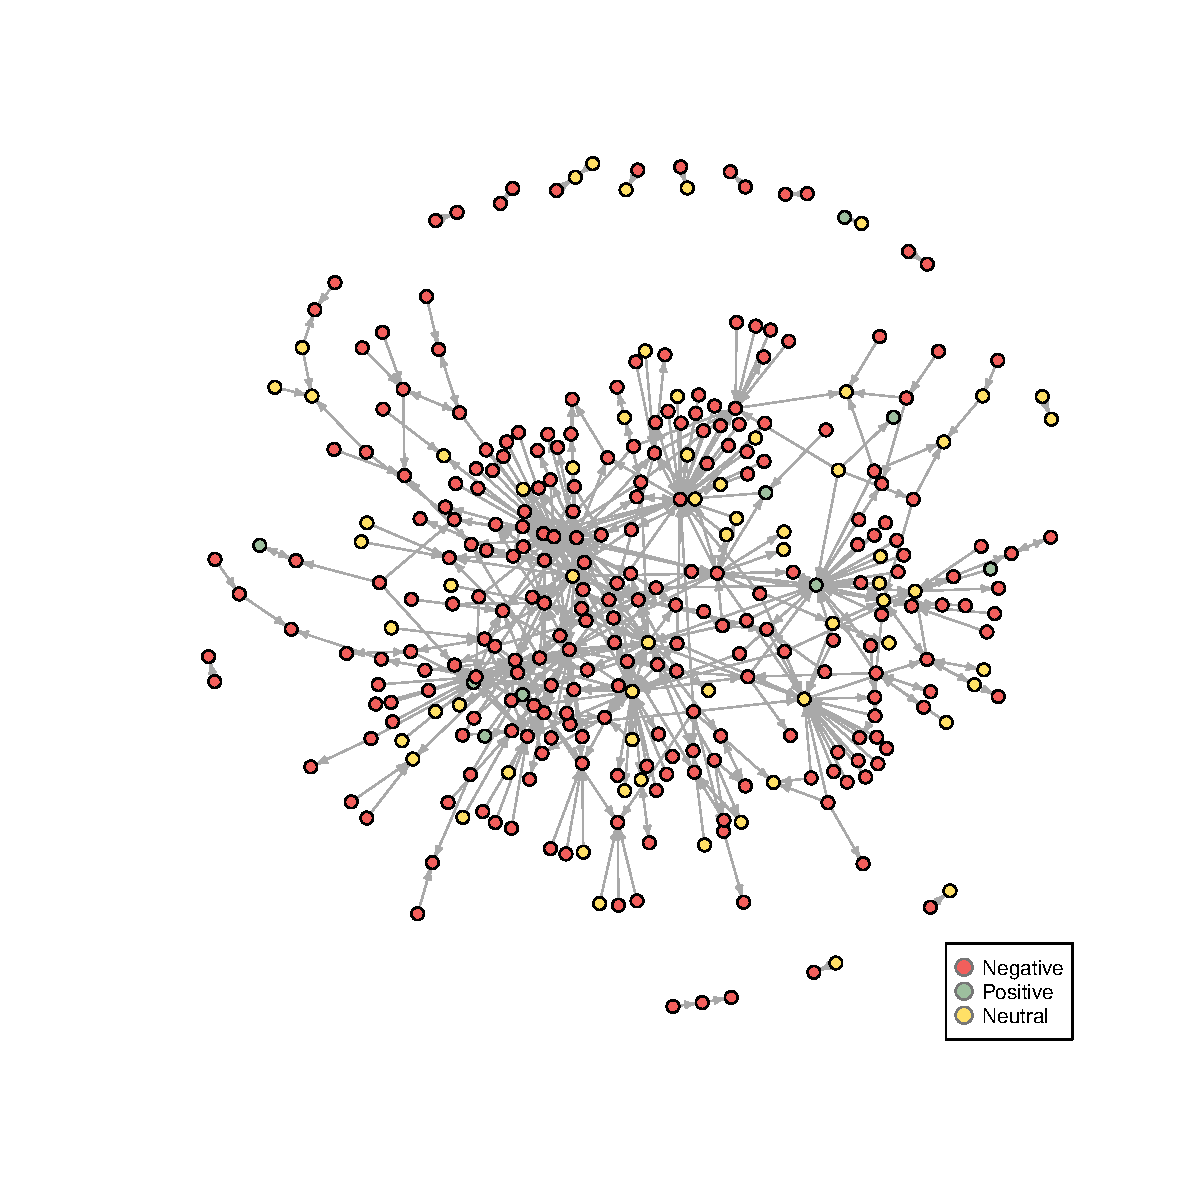
\includegraphics{SNA4DS_Report_files/figure-latex/main-network-plot-1} 

}

\caption{The plot of the network used for analysis. It shows the majority of the nodes labelled negative.}\label{fig:main-network-plot}
\end{figure}
\newpage

Furthermore, our data was initially a weighted network due to the potential for users to comment multiple times on each other's posts, adding complexity to our analysis. However, to simplify and focus on the presence of interactions rather than their frequency, we convert this into an unweighted network. This means we consider whether an interaction occurred between users, regardless of how often it happened.
Ultimately, we ended up with a network of 324 distinct actors interconnected through 553 ties, derived from comments posted between July 2023 and October 2023. This network is characterized by a notably low indegree and outdegree, as detailed in Figures \ref{fig:degree-in}, \ref{fig:degree-out}, pointing to its sparse connectivity.


\begin{figure}[!h]

{\centering 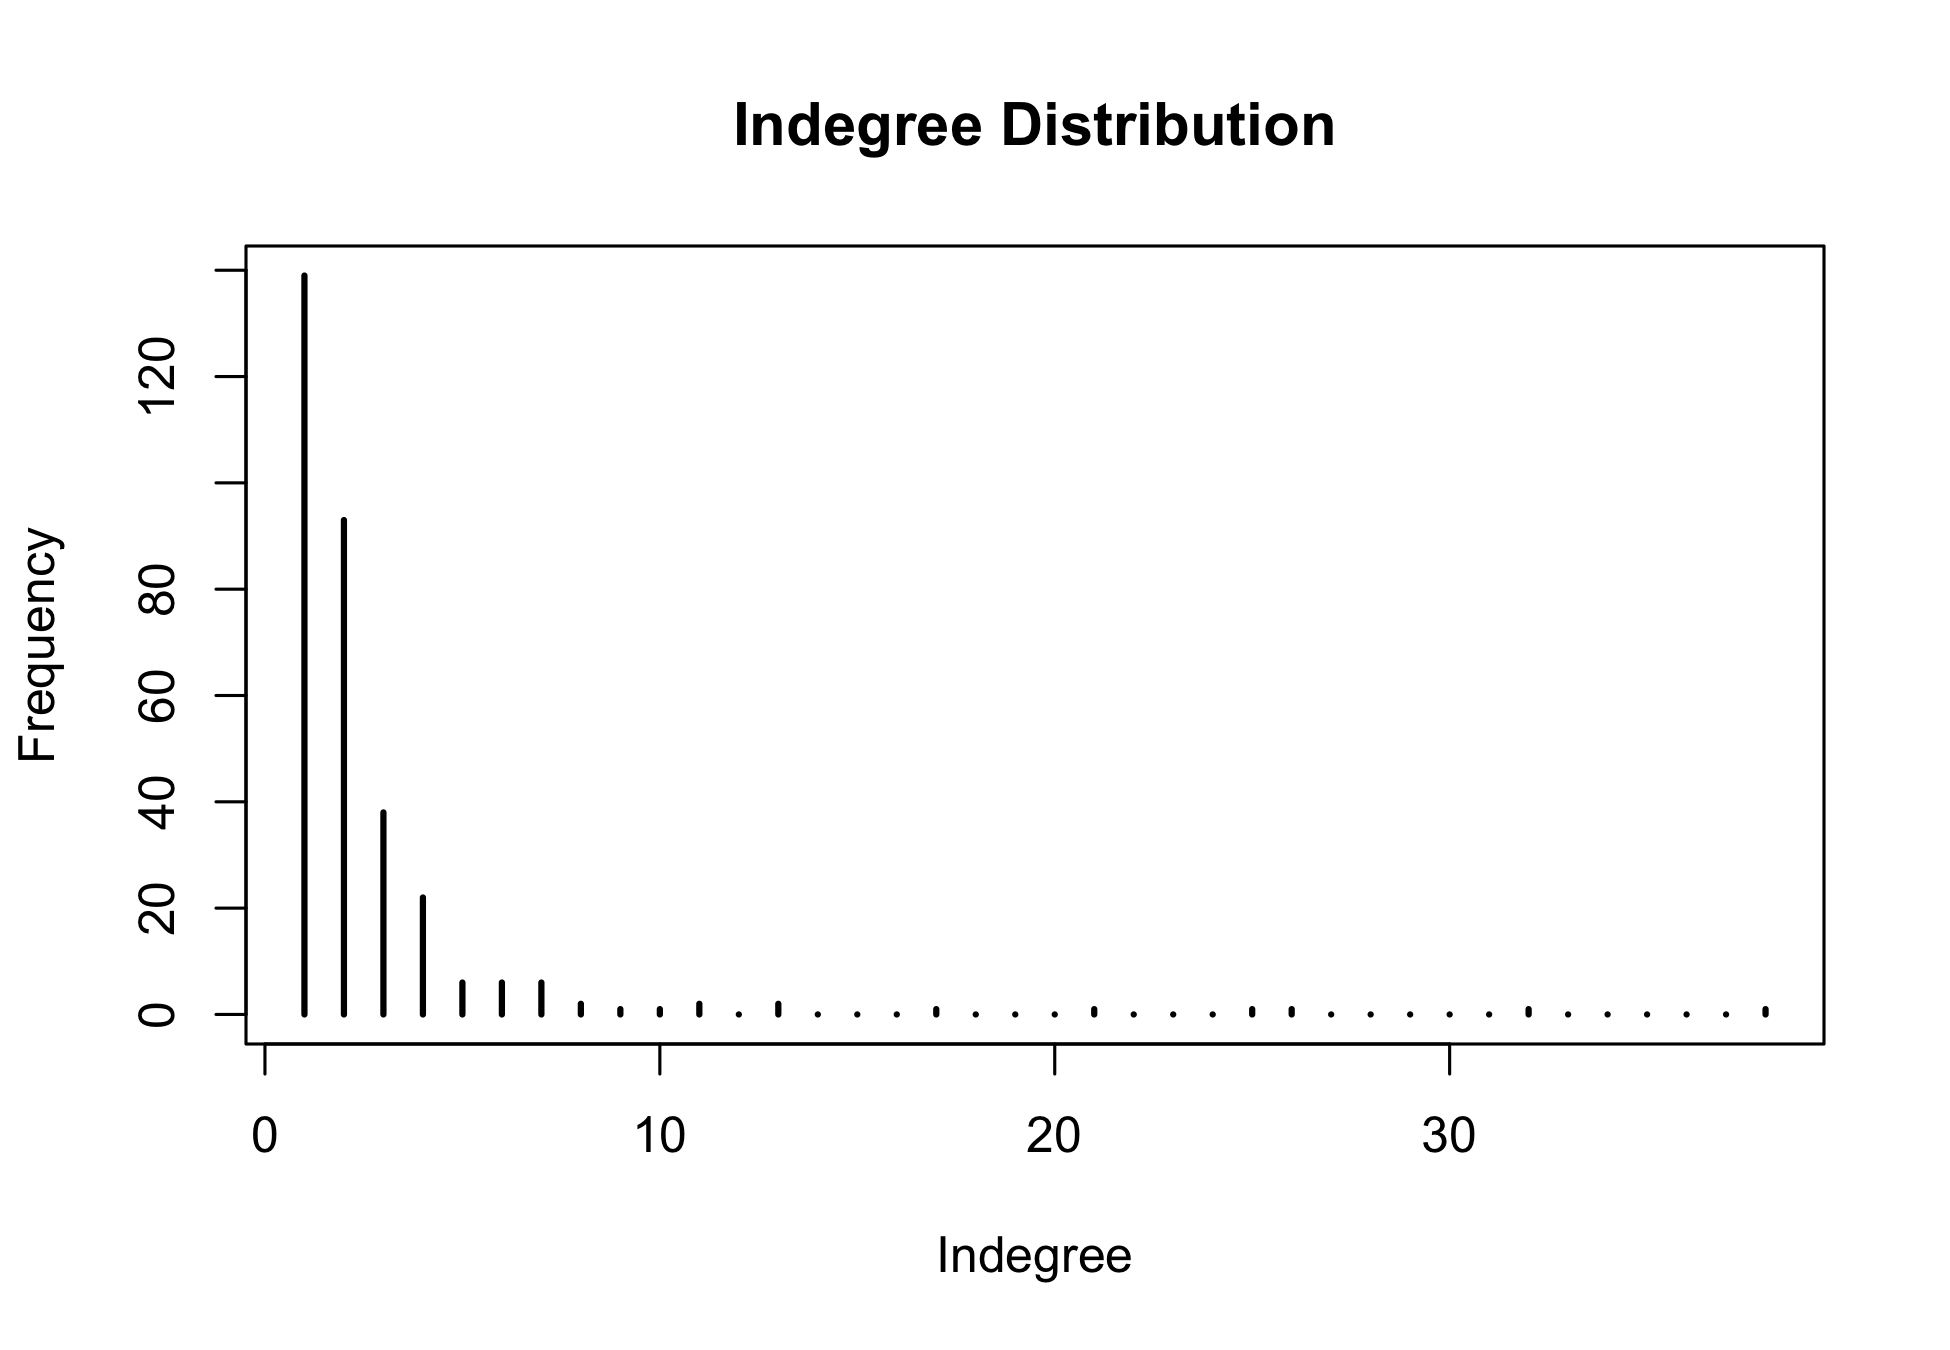
\includegraphics[width=0.5\linewidth,]{SNA4DS_Report_files/figure-latex/degree-in-1} 

}

\caption{The plot above shows the indegree distribution for the actors in the network.}\label{fig:degree-in}
\end{figure}



\begin{figure}[!h]

{\centering 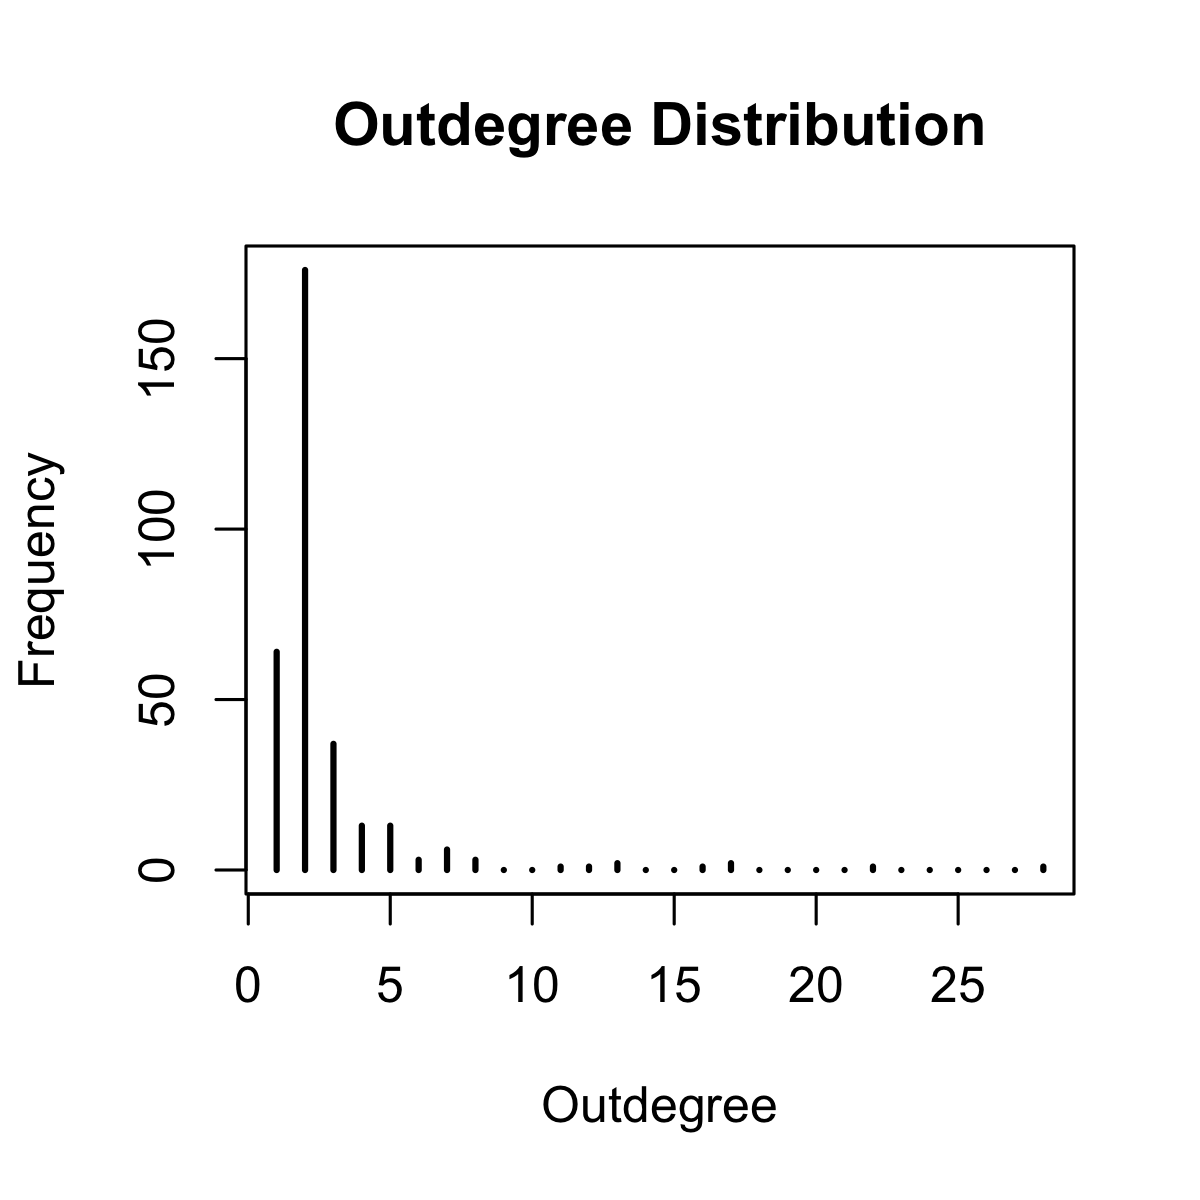
\includegraphics[width=0.5\linewidth,]{SNA4DS_Report_files/figure-latex/degree-out-1} 

}

\caption{The plot above shows the outdegree distribution for the actors in our network.}\label{fig:degree-out}
\end{figure}
\newpage

Additionally, Table \ref{tab:dyad-count-table} reveals that reciprocal interactions within this network are infrequent, while unidirectional interactions are more prevalent. The visual representation of the network, depicted in Figure \ref{fig:main-network-plot}, further highlights the sparse connectivity as we see a lot of isolated dyads. In this Figure \ref{fig:main-network-plot} a small subset of actors with significantly higher degrees of connectivity can also be found, an observation which underscores the relevance of our first study. The network descriptives can be found in Appendix A.\\
\strut \\



\begin{table}[!h]

\begin{center}
\begin{threeparttable}

\caption{\label{tab:dyad-count-table}An overview of the reciprocal dyads.}

\begin{tabular}{lll}
\toprule
Mutual & \multicolumn{1}{c}{Asymmetric} & \multicolumn{1}{c}{Null}\\
\midrule
70 & 413 & 51843\\
\bottomrule
\end{tabular}

\end{threeparttable}
\end{center}

\end{table}

\hfill\break

\subsubsection{\texorpdfstring{Potential Bias\\
}{Potential Bias }}\label{potential-bias}

Our research methodology, while comprehensive, is not without potential biases that could impact the interpretation of our results. The primary source of bias stems from Ongehoord Nederland as the sole YouTube channel for analysis. This channel's distinct right-wing orientation and ties to specific political ideologies may not represent the broader YouTube community or other political spectrums. Therefore, our findings, while indicative of echo chambers within this particular context, may not be generalizable to other YouTube channels or political orientations.
Another potential bias arises from our method of selecting videos. Although we chose a sequence of five videos randomly to increase the likelihood of finding users commenting on multiple videos, this approach might have inadvertently focused on a specific time frame or subset of topics, which may not encompass the full range of discussions typically found on the channel. This could limit the diversity of user interactions and viewpoints captured in our study.
It is crucial to acknowledge that these biases could influence the conclusions drawn from our study. The results should be interpreted with an understanding of these limitations and future research should aim to include a more diverse range of channels, video selection methods and user interaction types to provide a more comprehensive view of echo chambers on YouTube. This will help better understand online discourse's nuances and dynamics, especially in politically charged environments. \newpage

\subsection{Research Rationale}\label{research-rationale}

A shared understanding of `echo chambers' within social networks is essential to address our research questions effectively. Building upon Jasny et al. (2015) `s framework, we recognize echo chambers as social structures marked by significant homophily, where individuals sharing similar views are grouped together (Jasny et al., 2018, 2015; Jasny \& Fisher, 2019). This concept is encapsulated in the 'chamber', represented as a network configuration known as a transitive triad. In this configuration, information circulates from one actor (A) to another (C) both directly and via an intermediary (B), illustrating multiple paths of information flow within the same source and endpoint. In this `chamber,' a speaker, a mediating actor and a receiver are involved. Information in this configuration can travel directly from the speaker to the receiver or from the speaker through the mediating actor to the receiver. The similarity in content and sentiment of communications between actors with aligned opinions and outlooks identifies the 'echo' aspect. This phenomenon is visualized in Figure \ref{fig:echo-chamber-structure}.



\begin{figure}[H]

{\centering 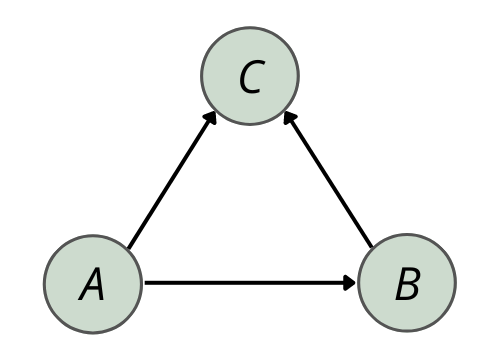
\includegraphics[width=1.67in,]{SNA4DS_Report_files/figures/transitive_triad_2} 

}

\caption{An echo chamber representation within the structural network configuration, also known as a transitive triad.}\label{fig:echo-chamber-structure}
\end{figure}

To assess the sentiment of a comment within a discussion section, we employed ChatGPT for zero-shot sentiment analysis. This analysis will categorize the comments of individual users as aligning with, being neutral toward, or opposing the political subject in question. ChatGPT will be used for sentiment analysis because it has shown remarkable zero-shot sentiment analysis proficiency, rivaling fine-tuned models such as BERT and state-of-the-art models trained with labeled data within their respective domains (Wang, Xie, Ding, Feng, \& Xia, 2023).
The sentiment focuses on the users' attitudes towards specific political entities, parties, politicians, policy issues and broader socio-cultural themes. This sentiment was categorized as positive, negative, or neutral, incorporating a nuanced understanding of the complexities and diversities inherent in the topics discussed:

\begin{enumerate}
    \item \textbf{Positive Sentiment:} This indicates approval, support, or positive feelings towards a subject. For instance, a comment expressing hope or confidence in a political movement is classified as positive.
    \item \textbf{Negative Sentiment:} This reflects dissatisfaction, disapproval, or negative emotions. Comments critical of political parties, policy decisions, or societal issues such as gender identity and LGBTQ+ topics are examples of negative sentiment.
    \item \textbf{Neutral Sentiment:} This denotes an objective, impartial, or moderate stance, devoid of strong positive or negative emotions, often informative in nature.
\end{enumerate}

This approach enables us to develop a more detailed understanding of public perception and sentiment about the different topics discussed in the comments. This assists in understanding and analyzing the complexity of public opinions and emotions in relation to these diverse subjects.
In assessing our hypothesis for our first research question we use CUGs because we cannot guarantee the normality assumptions required by many statistical tests. CUGs allows us to test our hypotheses despite the statistical complexities of the network representation. We use CUGs to determine whether centrality measures of our observed graph occur at levels exceeding what we would expect by chance. With centrality measures such as eigenvector centrality, degree centrality and betweenness centrality we aim to identify whether there are central players in our network. Eigenvector centrality is used to recognize influential nodes based not just on their direct connections, but more significantly on their connections to other highly connected and central nodes. Degree centrality is used to highlight nodes that have more connections, providing a measure of popularity. Betweenness centrality is included to identify nodes that act as bridges within the network structure, controlling the flow of information between other nodes.
For future research, methodologies such as the Multiple Regression Quadratic Assignment Procedure (MRQAP) may prove valuable for exploring how various attributes --- like subscriber count, number of likes, or number of comments --- are associated with centrality measures. Such an approach could contribute to our understanding of how certain attributes predict a node's likelihood of being a central figure.
Echoing the approach of Jasny et al. (2015), which focused on operationalizing the components of echo chambers in the US climate policy network, our second study also employs ERGMs (Jasny et al., 2015). ERGMs are ideal for this type of analysis due to its ability to comprehensively model complex social networks. It integrates both endogenous network effects and exogenous variables into a unified statistical framework, accurately capturing the intricate dynamics of social interactions (Cranmer, Desmarais, \& Morgan, 2020). This is important because this allows us to effectively analyze groups which are unified by shared sentiments. Additionally, ERGM's approach of treating the network as a single multivariate observation aligns well with our objective of empirically testing the structure and impact of echo chambers. \newpage

\section{\texorpdfstring{Results\\
}{Results }}\label{results}

\subsection{\texorpdfstring{Study 1\\
}{Study 1 }}\label{study-1}

In our first study, we aimed to investigate if the centralization observed in YouTube comment networks --- measured through eigenvector, degree and betweenness centrality --- was higher than what would be expected in a random scenario. This was analyzed using Conditional Uniform Graphs (CUGs), conditioned on the network's number of edges.\\
\strut \\


\begin{table}[h]

\begin{center}
\begin{threeparttable}

\caption{\label{tab:cug-results-table}P-values resulting from CUG Tests.}

\begin{tabular}{ll}
\toprule
centralization measure & \multicolumn{1}{c}{Pr(X>=Obs)}\\
\midrule
betweenness & 0.97\\
indegree & 0.00\\
outdegree & 0.00\\
eigenvector & 0.19\\
\bottomrule
\end{tabular}

\end{threeparttable}
\end{center}

\end{table}

The CUG results, presented in Table \ref{tab:cug-results-table}, provide insight into the network structure in terms of these centrality measures.
For both indegree and outdegree centrality, the findings were significant. A significant indegree centrality indicates that certain users in the network receive more interactions than others, highlighting the presence of particularly influential or attention-gathering users. Regarding outdegree centrality, the findings point to certain users being more active in initiating interactions or making connections within the network.
However, the situation is different for eigenvector centrality. Despite its high empirical value of 0.92, the result was not statistically significant. A high empirical value typically indicates a tendency for influential users within the network to be interconnected, suggesting the presence of clusters where influential users are more likely to be connected with each other. However, the non-significant result in this case means that such a tendency of influential users being connected is not different from what could happen in a random network.
The betweenness centrality also showed a non-significant result. This means that the network's nodes do not play a central role as intermediaries in the information flow compared to a random network. This indicates that while there are nodes that help in spreading information, their role is similar to what might occur randomly.

\subsection{\texorpdfstring{Study 2\\
}{Study 2 }}\label{study-2}

In this study, we analyse network formation based on the sentiment of user comments. Figure \ref{fig:ergm-results-plot-model5} presents the result of the ERGM from the best fitting model.\\
\strut \\


\begin{figure}[H]
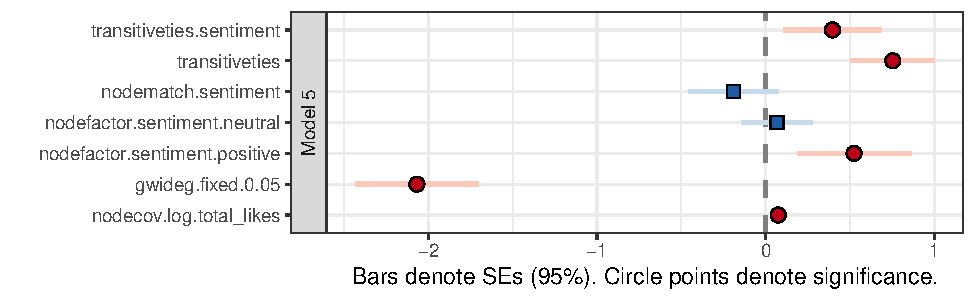
\includegraphics{SNA4DS_Report_files/figure-latex/ergm-results-plot-model5-1} \caption{ERGM results for model 5.}\label{fig:ergm-results-plot-model5}
\end{figure}

In our initial attempts to fit the model, we encountered challenges with achieving convergence. Our approach replicated the methodology used by Jasny et al. (2015), who also faced similar convergence issues. They resolved this by imposing constraints on the indegree distribution, a strategy we adopted as well. Implementing this constraint enabled our models to converge more effectively. However, it's important to note that we excluded the edges term from the model specification, as it is unfeasible to estimate it while constraining the indegree distribution. This adjustment alters the interpretation of our results, as the ERGM now shows how network structures deviate from what would be expected given the fixed indegree distribution.
We included a term for homophily, \textit{nodematch.sentiment}, to represent our `echo'. However, with a negative coefficient of -0.19 translating to a log odds of approximately 0.82, this term suggests that sharing the same sentiment inversely influences the formation of ties between two nodes. In other words, nodes with matching sentiments are slightly less likely to form ties than those with differing sentiments.
We also included transitive triads as a term, with \textit{transitiveties}, to represent the `chamber'. The positive coefficient of 0.75 for \textit{transitiveties}, translating to log odds of about 2.11, indicates a strong influence of transitive relationships in tie formation, irrespective of sentiment. This suggests that the presence of a transitive triad significantly increases the likelihood of tie formation within the network.
The full echo chamber mechanism is represented in the term \textit{transitiveties.sentiment}, with a positive coefficient of 0.4 and a corresponding log odds of approximately 1.49. The significance of both \textit{transitiveties.sentiment} and \textit{transitiveties} implies that the formation of transitive relationships is not due to chance and is influenced by the sentiment attribute. The positive coefficients here indicate a tendency for tie formation in scenarios where transitive relationships have similar sentiments.
It is also worth mentioning that \textit{nodefactor.sentiment.positive} is significant in our model, with a value of 0.52 translating to log odds of approximately 1.68. This finding highlights that comments characterized by positive sentiment are more inclined to establish connections within the network.
Lastly, the term \textit{nodecov.log.total\textunderscore like} is also significant with a coefficient of 0.07, which translates to log odds of approximately 1.07. This indicates that the total likes of an user is a significant predictor for the formation of ties within the network. This finding underscores the role of engagement, as measured by likes, in facilitating connections between nodes in the network. \newpage

\section{Discussion and Conclusion}\label{discussion-and-conclusion}

Our study aimed to investigate the existence of echo chambers on YouTube, a platform less studied in this context compared to others like Twitter. It also focuses on if there are prominent users as these could initiate or reinforce the echo chamber effects, which in turn contributes to polarization and ideological homogeneity. Our research has uncovered significant insights that not only enhance our theoretical understanding but also offer practical guidance for various stakeholders. Our approach was centered around two key research questions:

\textbf{RQ 1}
\emph{To what extent are prominent users present within YouTube channels' comment sections?}

\textbf{RQ 2}
\emph{To what extent are there echo chambers within YouTube channels' comment sections?}

Study 1 revealed that while some users are more prominent or active in the network (as shown by the indegree and indegree centrality), these users are not more likely to be connected to each other (eigenvector centrality) and their role as information brokers (betweenness centrality) are not significantly different from what might be seen in a random network. This suggests that while there are prominent users in terms of activity, they do not form a cohesive group of influencers or dominate the information brokerage within the network. Looking at the in degree centrality plot (figure plot) it's noticeable there relative high amount of non-negative sentiment nodes . In the discourse environment of the comment section this could possibly indicate an hostile environment for having a different opinion.
In Study 2, we found evidence supporting the existence of echo chambers on YouTube. The formation of transitive ties was also significant, indicating that these are not mere products of randomness. Important to note is that, contrary to the findings of Jasny et al. (2015), our study observed a lack of significant homophily. The lack of significant homophily within the YouTube comment networks, particularly in contrast to the homogeneous environment dominated by negative sentiments, could be partially explained by the insights from Study 1. As the central nodes do not seem to have an influential role in the network and the sentiments of nodes with high degrees seem to.
Another probable possibility could be due to the widespread negative sentiment in our network, making it difficult to observe homophily because most users share this sentiment. The lack of diverse sentiments in our network reduces the chances of forming distinct groups based on sentiment. Although this suggests our network is largely a single, homogeneous cluster, it does not rule out the possibility of smaller clusters forming based on other factors besides sentiment. It does suggest that one could describe our network as one big echo, in which chambers are being formed.
The findings contribute significantly to the theoretical understanding of social media dynamics as our research extends the concept of echo chambers beyond traditional platforms like Twitter and Facebook, demonstrating their presence in the unique context of YouTube. This contributes to the broader discourse on how digital platforms facilitate ideological segregation and polarization.
Understanding the role of prominent users and the dynamics of echo chambers is crucial for a range of stakeholders, including policymakers, educators and content creators. The study's findings can inform strategies to promote more balanced and diverse online conversations, thereby potentially mitigating the effects of polarization. These strategies could involve strengthening community guidelines, moderating content to prevent extremism, raising awareness about echo chambers and empowering users to diversify their content exposure.
For policymakers, these insights underscore the need for policies that foster diversity in online discourse and prevent platforms like YouTube from becoming hotbeds of extremism or misinformation. Educators and content creators can leverage these findings to promote critical thinking and digital literacy, equipping audiences to engage constructively in online environments.
The scope for future research is extensive and includes expanding the study to encompass a broader range of YouTube channels and political perspectives, conducting robustness checks for sentiment analysis and delving deeper into the characteristics of prominent users. Such research could provide a more nuanced understanding of user interactions and opinions, as discussed in Chapter 2, further enriching our knowledge of the dynamics at play in online echo chambers. It is also interesting to further research users with a high indegree as these individuals are likely to be influenced by the incoming interactions from other users, making them pivotal in the spread and reinforcement of ideas within echo chambers. Utilizing Temporal Exponential Random Graph Models could offer a dynamic view of how sentiments change over time within these networks. This approach could help identify users who are more susceptible to influence, thereby enabling the development of strategies to foster a more balanced and diverse discourse.
In conclusion, our research has revealed the complex dynamics of echo chambers on YouTube, highlighting the significant role of prominent users and the trend towards ideological homogeneity in the comment sections of politically oriented videos. These findings are critical in understanding the unique characteristics of social media platforms and their impact on public discourse and societal polarization. As digital platforms continue to evolve, the insights gained from our study can offer a roadmap for stakeholders in the digital space, aiding in the development of more informed and effective strategies to manage and comprehend the impact of social media on society. This study not only contributes to the academic discourse but also serves as a catalyst for action among policymakers, educators and content creators, steering us towards a more informed, balanced and cohesive digital world.

\newpage

\section*{References}\label{references}
\addcontentsline{toc}{section}{References}

\begingroup
\setlength{\parindent}{-0.5in}
\setlength{\leftskip}{0.5in}

\phantomsection\label{refs}
\begin{CSLReferences}{1}{0}
\bibitem[\citeproctext]{ref-cinelli2021echo}
Cinelli, M., De Francisci Morales, G., Galeazzi, A., Quattrociocchi, W., \& Starnini, M. (2021). The echo chamber effect on social media. \emph{Proceedings of the National Academy of Sciences}, \emph{118}(9), e2023301118.

\bibitem[\citeproctext]{ref-colleoni2014echo}
Colleoni, E., Rozza, A., \& Arvidsson, A. (2014). Echo chamber or public sphere? Predicting political orientation and measuring political homophily in twitter using big data. \emph{Journal of Communication}, \emph{64}(2), 317--332.

\bibitem[\citeproctext]{ref-cranmer2020inferential}
Cranmer, S. J., Desmarais, B. A., \& Morgan, J. W. (2020). \emph{Inferential network analysis}. Cambridge University Press.

\bibitem[\citeproctext]{ref-du2017echo}
Du, S., \& Gregory, S. (2017). The echo chamber effect in twitter: Does community polarization increase? \emph{Complex Networks \& Their Applications v: Proceedings of the 5th International Workshop on Complex Networks and Their Applications (COMPLEX NETWORKS 2016)}, 373--378. Springer.

\bibitem[\citeproctext]{ref-grusauskaite2023debating}
Grusauskaite, K., Carbone, L., Harambam, J., \& Aupers, S. (2023). Debating (in) echo chambers: How culture shapes communication in conspiracy theory networks on YouTube. \emph{New Media \& Society}, 14614448231162585.

\bibitem[\citeproctext]{ref-hosseinmardi2020evaluating}
Hosseinmardi, H., Ghasemian, A., Clauset, A., Rothschild, D. M., Mobius, M., \& Watts, D. J. (2020). Evaluating the scale, growth, and origins of right-wing echo chambers on YouTube. \emph{arXiv Preprint arXiv:2011.12843}.

\bibitem[\citeproctext]{ref-jasny2018shifting}
Jasny, L., Dewey, A. M., Robertson, A. G., Yagatich, W., Dubin, A. H., Waggle, J. M., \& Fisher, D. R. (2018). Shifting echo chambers in US climate policy networks. \emph{PloS One}, \emph{13}(9), e0203463.

\bibitem[\citeproctext]{ref-jasny2019echo}
Jasny, L., \& Fisher, D. R. (2019). Echo chambers in climate science. \emph{Environmental Research Communications}, \emph{1}(10), 101003.

\bibitem[\citeproctext]{ref-jasny2015empirical}
Jasny, L., Waggle, J., \& Fisher, D. R. (2015). An empirical examination of echo chambers in US climate policy networks. \emph{Nature Climate Change}, \emph{5}(8), 782--786.

\bibitem[\citeproctext]{ref-levy2019echo}
Levy, G., \& Razin, R. (2019). Echo chambers and their effects on economic and political outcomes. \emph{Annual Review of Economics}, \emph{11}, 303--328.

\bibitem[\citeproctext]{ref-mccoy2019toward}
McCoy, J., \& Somer, M. (2019). Toward a theory of pernicious polarization and how it harms democracies: Comparative evidence and possible remedies. \emph{The Annals of the American Academy of Political and Social Science}, \emph{681}(1), 234--271.

\bibitem[\citeproctext]{ref-rochert2020opinion}
Röchert, D., Neubaum, G., Ross, B., Brachten, F., \& Stieglitz, S. (2020). Opinion-based homogeneity on YouTube: Combining sentiment and social network analysis. \emph{Computational Communication Research}, \emph{2}(1), 81--108.

\bibitem[\citeproctext]{ref-sung2013influence}
Sung, J., Moon, S., \& Lee, J.-G. (2013). The influence in twitter: Are they really influenced? \emph{International Workshop on Behavior and Social Informatics and Computing}, 95--105. Springer.

\bibitem[\citeproctext]{ref-villa2021echo}
Villa, G., Pasi, G., \& Viviani, M. (2021). Echo chamber detection and analysis: A topology-and content-based approach in the COVID-19 scenario. \emph{Social Network Analysis and Mining}, \emph{11}(1), 78.

\bibitem[\citeproctext]{ref-wang2023chatgpt}
Wang, Z., Xie, Q., Ding, Z., Feng, Y., \& Xia, R. (2023). Is ChatGPT a good sentiment analyzer? A preliminary study. \emph{arXiv Preprint arXiv:2304.04339}.

\bibitem[\citeproctext]{ref-wattenhofer2012youtube}
Wattenhofer, M., Wattenhofer, R., \& Zhu, Z. (2012). The YouTube social network. \emph{Proceedings of the International AAAI Conference on Web and Social Media}, \emph{6}, 354--361.

\bibitem[\citeproctext]{ref-wittenberg2021minimal}
Wittenberg, C., Tappin, B. M., Berinsky, A. J., \& Rand, D. G. (2021). The (minimal) persuasive advantage of political video over text. \emph{Proceedings of the National Academy of Sciences}, \emph{118}(47), e2114388118.

\bibitem[\citeproctext]{ref-YouTube2022Handles}
YouTube. (2022). \emph{Announcing YouTube handles: A unique identifier to discover and connect on YouTube}. \url{https://support.google.com/youtube/thread/183284252}.

\end{CSLReferences}

\endgroup

\newpage

\section*{Appendix A}\label{appendix-a}
\addcontentsline{toc}{section}{Appendix A}

This first appendix includes all of the R chunks of code that were hidden throughout the document to help with reproducibility readibility and/or setup.

\textbf{R set-up code}

\begin{Shaded}
\begin{Highlighting}[]
\FunctionTok{library}\NormalTok{(}\StringTok{"papaja"}\NormalTok{)}
\FunctionTok{r\_refs}\NormalTok{(}\StringTok{"r{-}references.bib"}\NormalTok{)}
\NormalTok{knitr}\SpecialCharTok{::}\NormalTok{opts\_chunk}\SpecialCharTok{$}\FunctionTok{set}\NormalTok{(}\AttributeTok{fig.pos =} \StringTok{"H"}\NormalTok{, }\AttributeTok{out.extra =} \StringTok{""}\NormalTok{, }
                      \AttributeTok{echo =} \ConstantTok{FALSE}\NormalTok{, }\AttributeTok{cache =} \ConstantTok{TRUE}\NormalTok{)}

\FunctionTok{setwd}\NormalTok{(}\StringTok{"../data\_preparation/prepared\_data"}\NormalTok{)}
\NormalTok{graph }\OtherTok{\textless{}{-}}\NormalTok{ igraph}\SpecialCharTok{::}\FunctionTok{read\_graph}\NormalTok{(}
  \AttributeTok{file =} \StringTok{"network.graphml"}\NormalTok{,}
  \AttributeTok{format =} \StringTok{"graphml"}
\NormalTok{)}

\CommentTok{\# Loading environments with our data}
\FunctionTok{setwd}\NormalTok{(}\StringTok{"../../data\_analysis"}\NormalTok{)}
\FunctionTok{load}\NormalTok{(}\StringTok{"model\_results.RData"}\NormalTok{)}
\end{Highlighting}
\end{Shaded}

\begin{Shaded}
\begin{Highlighting}[]
\CommentTok{\# Seed for random number generation}
\FunctionTok{set.seed}\NormalTok{(}\DecValTok{42}\NormalTok{)}
\NormalTok{knitr}\SpecialCharTok{::}\NormalTok{opts\_chunk}\SpecialCharTok{$}\FunctionTok{set}\NormalTok{(}\AttributeTok{cache.extra =}\NormalTok{ knitr}\SpecialCharTok{::}\NormalTok{rand\_seed)}
\end{Highlighting}
\end{Shaded}

\textbf{R code for plots and tables}

\begin{Shaded}
\begin{Highlighting}[]
\CommentTok{\# Code for plotting the network}
\NormalTok{igraph}\SpecialCharTok{::}\FunctionTok{V}\NormalTok{(graph)}\SpecialCharTok{$}\NormalTok{color }\OtherTok{\textless{}{-}} \StringTok{"black"}
\NormalTok{igraph}\SpecialCharTok{::}\FunctionTok{V}\NormalTok{(graph) [ sentiment }\SpecialCharTok{==} \StringTok{\textquotesingle{}negative\textquotesingle{}}\NormalTok{ ]}\SpecialCharTok{$}\NormalTok{color }\OtherTok{\textless{}{-}} \StringTok{"\#F25F5C"}
\NormalTok{igraph}\SpecialCharTok{::}\FunctionTok{V}\NormalTok{(graph) [ sentiment }\SpecialCharTok{==} \StringTok{\textquotesingle{}positive\textquotesingle{}}\NormalTok{ ]}\SpecialCharTok{$}\NormalTok{color }\OtherTok{\textless{}{-}} \StringTok{"\#9DBF9E"}
\NormalTok{igraph}\SpecialCharTok{::}\FunctionTok{V}\NormalTok{(graph) [ sentiment }\SpecialCharTok{==} \StringTok{\textquotesingle{}neutral\textquotesingle{}}\NormalTok{ ]}\SpecialCharTok{$}\NormalTok{color }\OtherTok{\textless{}{-}} \StringTok{"\#FFE066"}

\FunctionTok{plot}\NormalTok{(}
\NormalTok{  graph,}
  \AttributeTok{vertex.label =} \ConstantTok{NA}\NormalTok{,}
  \AttributeTok{edge.arrow.size =}\NormalTok{ .}\DecValTok{35}\NormalTok{,}
  \AttributeTok{vertex.size =} \DecValTok{3}\NormalTok{,}
  \AttributeTok{vertex.color =}\NormalTok{ igraph}\SpecialCharTok{::}\FunctionTok{V}\NormalTok{(graph)}\SpecialCharTok{$}\NormalTok{color}
\NormalTok{)}

\NormalTok{colrs }\OtherTok{\textless{}{-}} \FunctionTok{c}\NormalTok{(}\StringTok{"\#F25F5C"}\NormalTok{,}\StringTok{"\#9DBF9E"}\NormalTok{,}\StringTok{"\#FFE066"}\NormalTok{)}
\NormalTok{graphics}\SpecialCharTok{::}\FunctionTok{legend}\NormalTok{(}\AttributeTok{x =} \FloatTok{0.75}\NormalTok{, }\AttributeTok{y =} \SpecialCharTok{{-}}\NormalTok{.}\DecValTok{85}\NormalTok{, }\FunctionTok{c}\NormalTok{(}\StringTok{"Negative"}\NormalTok{,}\StringTok{"Positive"}\NormalTok{,}\StringTok{"Neutral"}\NormalTok{), }
                 \AttributeTok{pch =} \DecValTok{21}\NormalTok{, }\AttributeTok{col =} \StringTok{"\#777777"}\NormalTok{, }\AttributeTok{pt.bg =}\NormalTok{ colrs, }\AttributeTok{pt.cex =} \FloatTok{1.5}\NormalTok{, }
                 \AttributeTok{cex =}\NormalTok{ .}\DecValTok{8}\NormalTok{, }\AttributeTok{bty =} \StringTok{"o"}\NormalTok{, }\AttributeTok{ncol =} \DecValTok{1}\NormalTok{)}
\end{Highlighting}
\end{Shaded}

\begin{Shaded}
\begin{Highlighting}[]
\CommentTok{\# Code for plotting the indegree distribution}
\NormalTok{degree\_distribution\_in }\OtherTok{\textless{}{-}}\NormalTok{ snafun}\SpecialCharTok{::}\FunctionTok{g\_degree\_distribution}\NormalTok{(graph, }
                                                        \AttributeTok{mode =} \StringTok{"in"}\NormalTok{, }
                                                        \AttributeTok{type =} \StringTok{"count"}
\NormalTok{                                                        )}
\CommentTok{\# Create a frequency plot with lines}
\FunctionTok{plot}\NormalTok{(}\DecValTok{1}\SpecialCharTok{:}\FunctionTok{length}\NormalTok{(degree\_distribution\_in), degree\_distribution\_in, }\AttributeTok{type =} \StringTok{"h"}\NormalTok{, }
     \AttributeTok{lwd =} \DecValTok{2}\NormalTok{, }\AttributeTok{main =} \StringTok{"Indegree Distribution"}\NormalTok{,}
     \AttributeTok{xlab =} \StringTok{"Indegree"}\NormalTok{, }\AttributeTok{ylab =} \StringTok{"Frequency"}\NormalTok{)}
\end{Highlighting}
\end{Shaded}

\begin{Shaded}
\begin{Highlighting}[]
\CommentTok{\# Code for plotting the outdegree distribution}
\NormalTok{degree\_distribution\_out }\OtherTok{\textless{}{-}}\NormalTok{ snafun}\SpecialCharTok{::}\FunctionTok{g\_degree\_distribution}\NormalTok{(graph, }
                                                         \AttributeTok{mode =} \StringTok{"out"}\NormalTok{, }
                                                         \AttributeTok{type =} \StringTok{"count"}
\NormalTok{                                                         )}

\CommentTok{\# Create a frequency plot with lines}
\FunctionTok{plot}\NormalTok{(}\DecValTok{1}\SpecialCharTok{:}\FunctionTok{length}\NormalTok{(degree\_distribution\_out), degree\_distribution\_out, }\AttributeTok{type =} \StringTok{"h"}\NormalTok{, }
     \AttributeTok{lwd =} \DecValTok{2}\NormalTok{, }\AttributeTok{main =} \StringTok{"Outdegree Distribution"}\NormalTok{, }
     \AttributeTok{xlab =} \StringTok{"Outdegree"}\NormalTok{, }\AttributeTok{ylab =} \StringTok{"Frequency"}\NormalTok{)}
\end{Highlighting}
\end{Shaded}

\begin{Shaded}
\begin{Highlighting}[]
\CommentTok{\# code for plotting the dyad count table}
\NormalTok{dyad\_count }\OtherTok{\textless{}{-}}\NormalTok{ snafun}\SpecialCharTok{::}\FunctionTok{count\_dyads}\NormalTok{(graph, }\AttributeTok{echo =} \ConstantTok{FALSE}\NormalTok{)}
\FunctionTok{apa\_table}\NormalTok{(dyad\_count,}
          \AttributeTok{placement =} \StringTok{"!h"}\NormalTok{,}
          \AttributeTok{caption =} \StringTok{"(ref:dyad{-}count{-}table)"}\NormalTok{)}
\end{Highlighting}
\end{Shaded}

\begin{Shaded}
\begin{Highlighting}[]
\CommentTok{\# Reading file from figures directory}
\NormalTok{knitr}\SpecialCharTok{::}\FunctionTok{include\_graphics}\NormalTok{(}
  \StringTok{"SNA4DS\_Report\_files/figures/transitive\_triad\_2.png"}
\NormalTok{  )}
\end{Highlighting}
\end{Shaded}

\begin{Shaded}
\begin{Highlighting}[]
\FunctionTok{apa\_table}\NormalTok{(cug\_results,}
          \AttributeTok{placement =} \StringTok{"h"}\NormalTok{,}
          \AttributeTok{caption =} \StringTok{"(ref:cug{-}results{-}table)"}\NormalTok{)}
\end{Highlighting}
\end{Shaded}

\newpage

\section*{Appendix B}\label{appendix-b}
\addcontentsline{toc}{section}{Appendix B}



\begin{Shaded}
\begin{Highlighting}[]
\NormalTok{centralities\_plot }\OtherTok{\textless{}{-}}\NormalTok{ snafun}\SpecialCharTok{::}\FunctionTok{plot\_centralities}\NormalTok{(}
\NormalTok{  graph,}
  \AttributeTok{measures =} \FunctionTok{c}\NormalTok{(}\StringTok{"betweenness"}\NormalTok{, }\StringTok{"closeness"}\NormalTok{, }\StringTok{"degree"}\NormalTok{, }\StringTok{"eccentricity"}\NormalTok{), }
  \AttributeTok{directed =} \ConstantTok{TRUE}\NormalTok{,}
  \AttributeTok{mode =} \StringTok{"all"}\NormalTok{,}
  \AttributeTok{k =} \DecValTok{3}\NormalTok{,}
  \AttributeTok{rescaled =} \ConstantTok{FALSE}
\NormalTok{)}
\end{Highlighting}
\end{Shaded}

\begin{figure}[H]
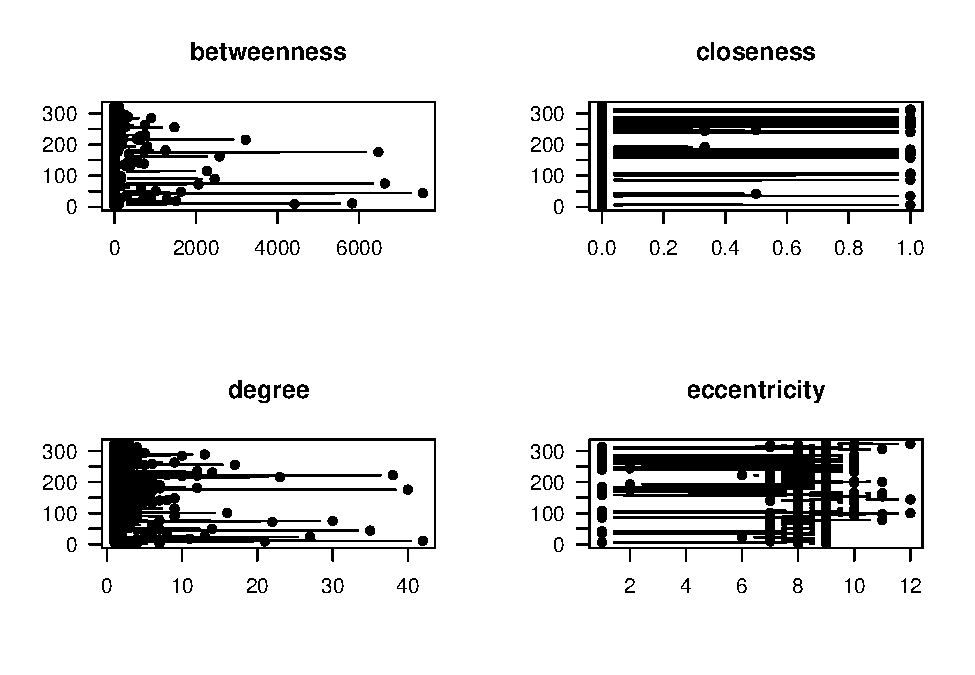
\includegraphics{SNA4DS_Report_files/figure-latex/centralities-plot-1} \caption{The centrality scores for each node in our network plotted.}\label{fig:centralities-plot}
\end{figure}



\begin{Shaded}
\begin{Highlighting}[]
\CommentTok{\# Plotting indegree for each node }
\CommentTok{\# Coloring each node based on its sentiment}
\NormalTok{igraph}\SpecialCharTok{::}\FunctionTok{V}\NormalTok{(graph)}\SpecialCharTok{$}\NormalTok{color }\OtherTok{\textless{}{-}} \StringTok{"orange"}
\NormalTok{igraph}\SpecialCharTok{::}\FunctionTok{V}\NormalTok{(graph) [ sentiment }\SpecialCharTok{==} \StringTok{\textquotesingle{}negative\textquotesingle{}}\NormalTok{ ]}\SpecialCharTok{$}\NormalTok{color }\OtherTok{\textless{}{-}} \StringTok{"\#F25F5C"}
\NormalTok{igraph}\SpecialCharTok{::}\FunctionTok{V}\NormalTok{(graph) [ sentiment }\SpecialCharTok{==} \StringTok{\textquotesingle{}positive\textquotesingle{}}\NormalTok{ ]}\SpecialCharTok{$}\NormalTok{color }\OtherTok{\textless{}{-}} \StringTok{"\#9DBF9E"}
\NormalTok{igraph}\SpecialCharTok{::}\FunctionTok{V}\NormalTok{(graph) [ sentiment }\SpecialCharTok{==} \StringTok{\textquotesingle{}neutral\textquotesingle{}}\NormalTok{ ]}\SpecialCharTok{$}\NormalTok{color }\OtherTok{\textless{}{-}} \StringTok{"orange"}

\NormalTok{my\_df }\OtherTok{\textless{}{-}} \FunctionTok{data.frame}\NormalTok{(}
\NormalTok{  igraph}\SpecialCharTok{::}\FunctionTok{get.vertex.attribute}\NormalTok{(graph, }\AttributeTok{name =} \StringTok{"id"}\NormalTok{), }
\NormalTok{  igraph}\SpecialCharTok{::}\FunctionTok{get.vertex.attribute}\NormalTok{(graph, }\AttributeTok{name =} \StringTok{"color"}\NormalTok{),}
  \DecValTok{1}\SpecialCharTok{:}\DecValTok{324}
\NormalTok{  )}

\NormalTok{v\_degree }\OtherTok{\textless{}{-}}\NormalTok{ igraph}\SpecialCharTok{::}\FunctionTok{degree}\NormalTok{(graph, }\AttributeTok{mode =} \StringTok{"in"}\NormalTok{)}

\NormalTok{my\_df }\OtherTok{\textless{}{-}} \FunctionTok{cbind}\NormalTok{(my\_df, v\_degree)}

\FunctionTok{names}\NormalTok{(my\_df) }\OtherTok{\textless{}{-}} \FunctionTok{c}\NormalTok{(}\StringTok{"id"}\NormalTok{, }\StringTok{"color"}\NormalTok{, }\StringTok{"new\_id"}\NormalTok{, }\StringTok{"degree"}\NormalTok{)}

\FunctionTok{plot}\NormalTok{(}\AttributeTok{y =}\NormalTok{ my\_df}\SpecialCharTok{$}\NormalTok{new\_id, }
     \AttributeTok{x =}\NormalTok{ my\_df}\SpecialCharTok{$}\NormalTok{degree,}
     \AttributeTok{xlab =} \StringTok{"indegree"}\NormalTok{,}
     \AttributeTok{ylab =}\StringTok{""}\NormalTok{,}
     \AttributeTok{col =}\NormalTok{ my\_df}\SpecialCharTok{$}\NormalTok{color,}
     \AttributeTok{type =} \StringTok{"b"}\NormalTok{,}
     \AttributeTok{pch =} \DecValTok{16}\NormalTok{)}

\CommentTok{\# Adding a legend}
\FunctionTok{legend}\NormalTok{(}\StringTok{"topright"}\NormalTok{, }\CommentTok{\# Location of the legend. Change as needed.}
       \AttributeTok{legend =} \FunctionTok{c}\NormalTok{(}\StringTok{"Negative: 253"}\NormalTok{, }
                  \StringTok{"Positive: 6"}\NormalTok{, }
                  \StringTok{"Neutral: 62"}\NormalTok{),  }\CommentTok{\# Labels in the legend}
       \AttributeTok{col =} \FunctionTok{c}\NormalTok{(}\StringTok{"\#F25F5C"}\NormalTok{, }
               \StringTok{"\#9DBF9E"}\NormalTok{, }
               \StringTok{"orange"}\NormalTok{), }\CommentTok{\# Colors corresponding to labels}
       \AttributeTok{pch =} \DecValTok{16}\NormalTok{)}
\end{Highlighting}
\end{Shaded}

\begin{figure}[H]
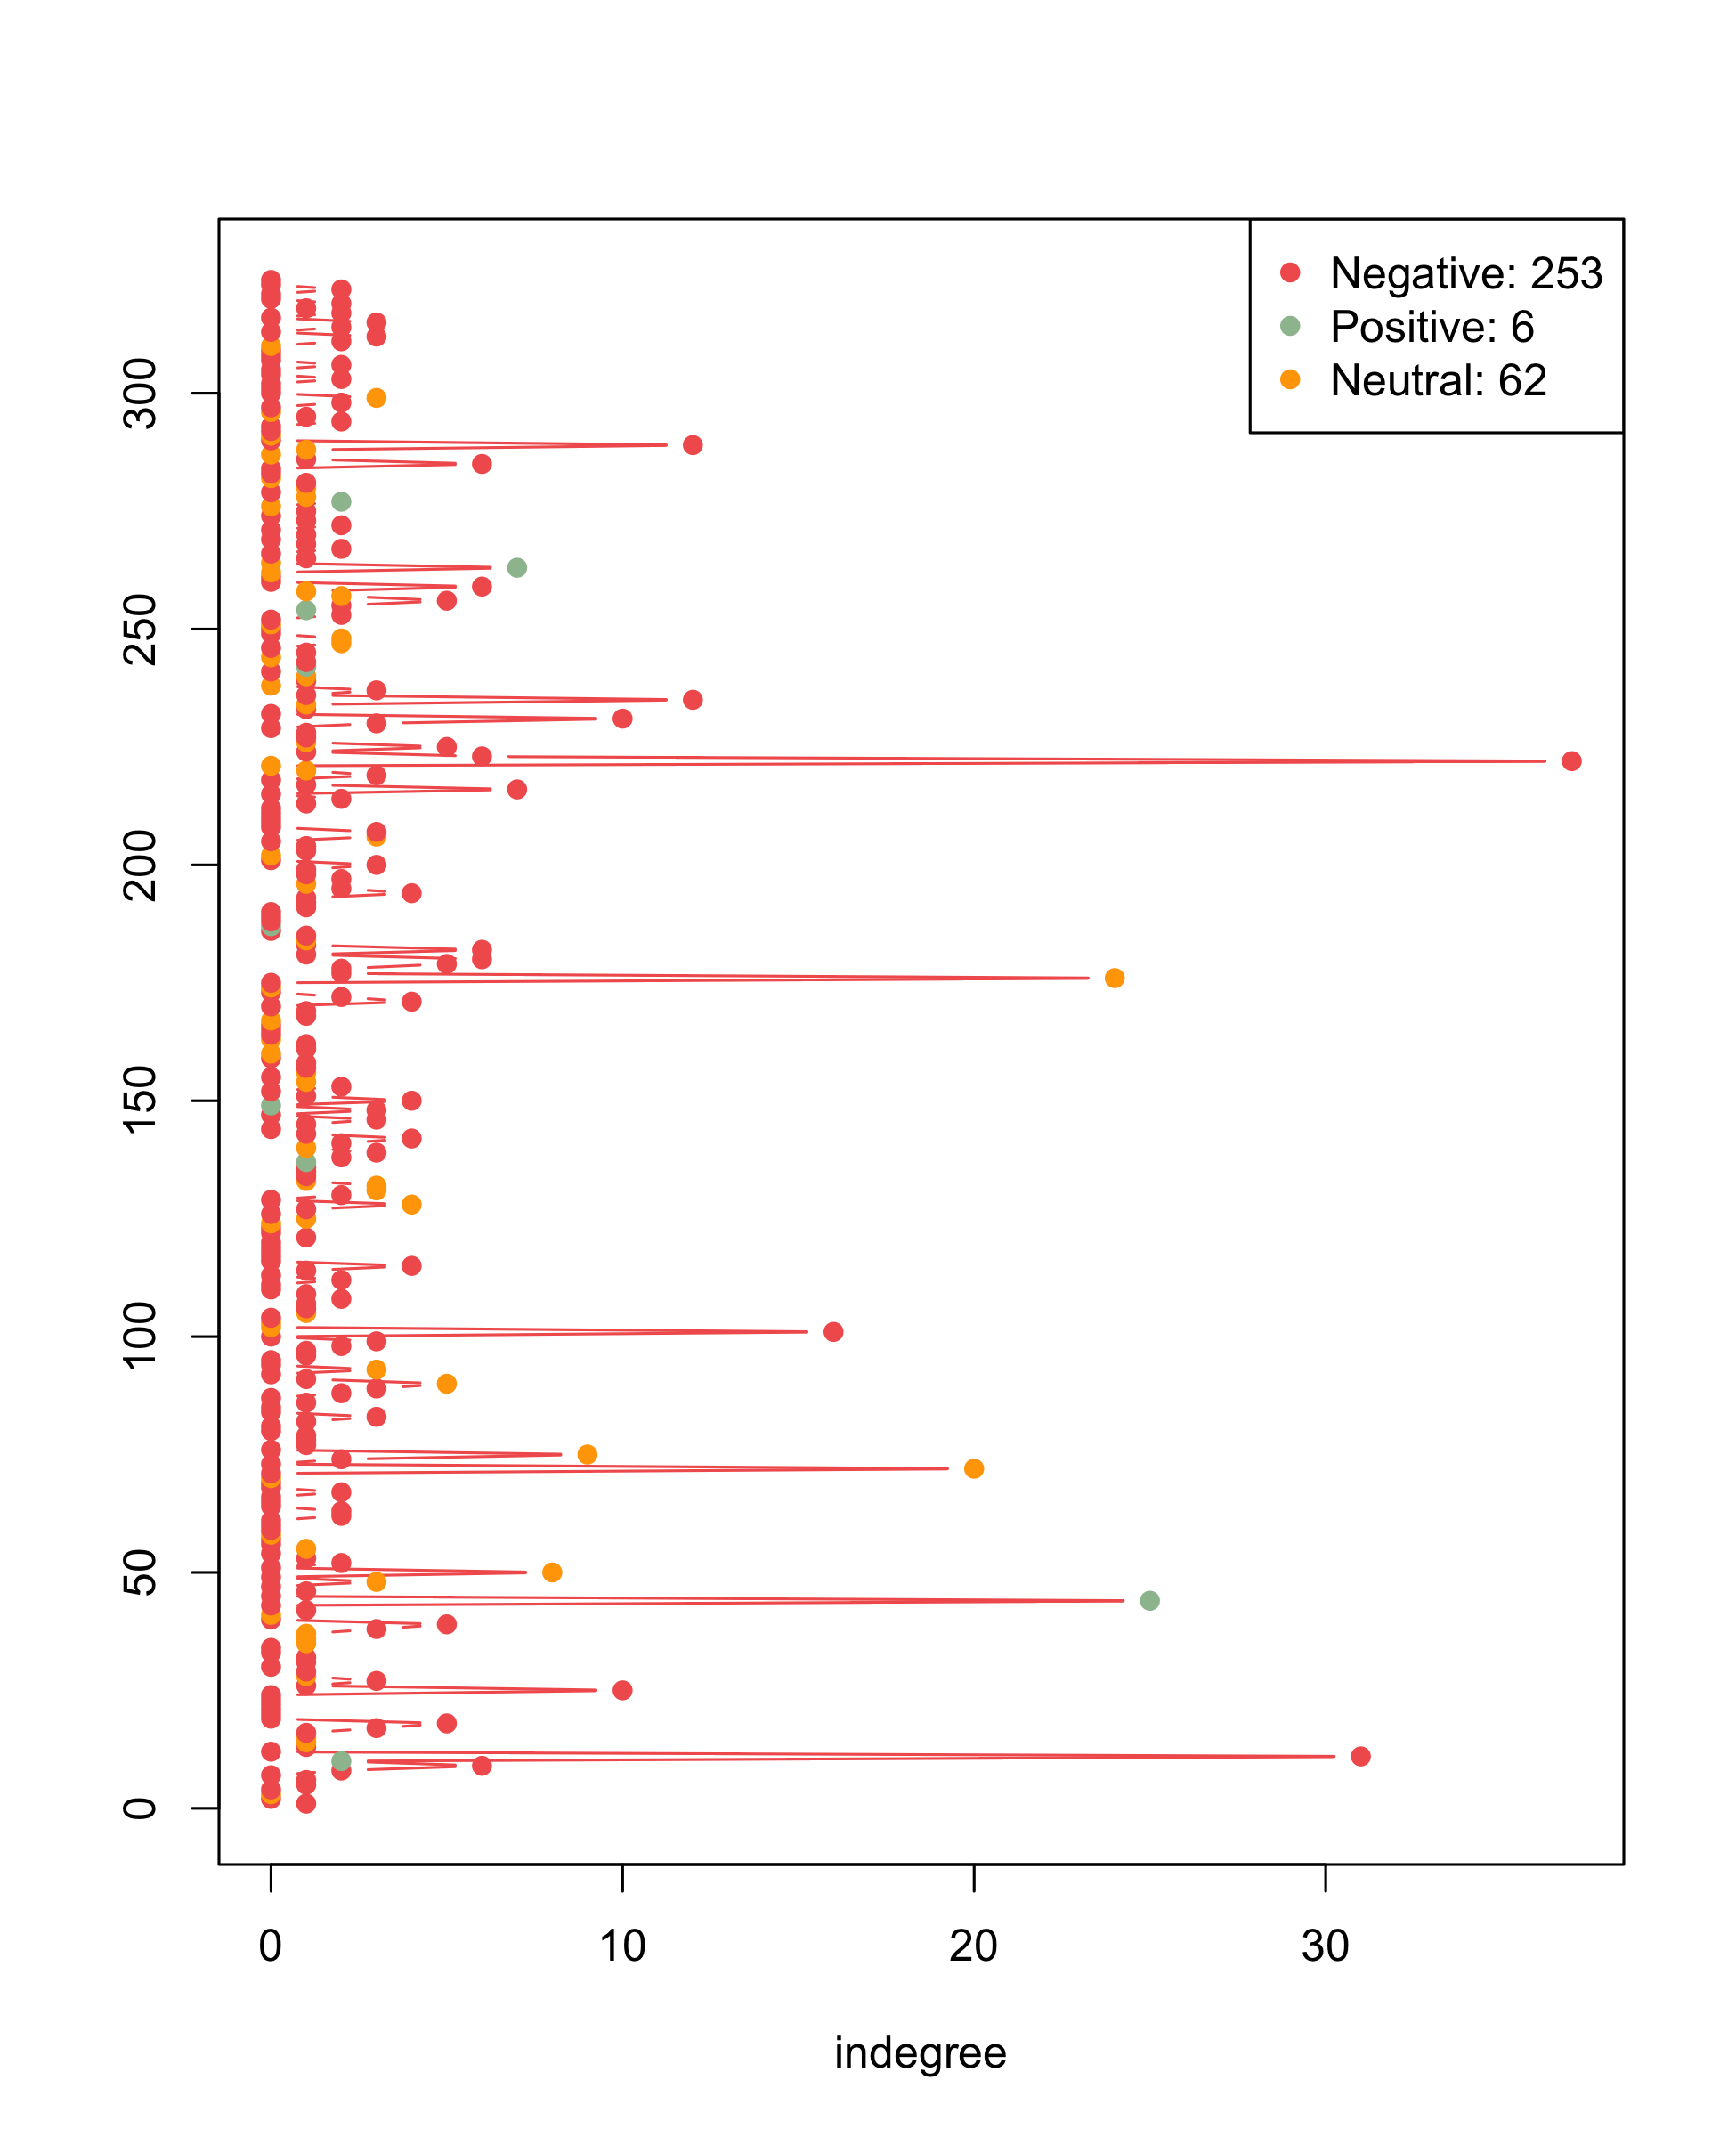
\includegraphics{SNA4DS_Report_files/figure-latex/indegree-plot-1} \caption{The indegree plotted for each node in the network}\label{fig:indegree-plot}
\end{figure}



\begin{Shaded}
\begin{Highlighting}[]
\CommentTok{\# Plotting outdegree for each node }
\CommentTok{\# Coloring each node based on its sentiment}
\NormalTok{igraph}\SpecialCharTok{::}\FunctionTok{V}\NormalTok{(graph)}\SpecialCharTok{$}\NormalTok{color }\OtherTok{\textless{}{-}} \StringTok{"orange"}
\NormalTok{igraph}\SpecialCharTok{::}\FunctionTok{V}\NormalTok{(graph) [ sentiment }\SpecialCharTok{==} \StringTok{\textquotesingle{}negative\textquotesingle{}}\NormalTok{ ]}\SpecialCharTok{$}\NormalTok{color }\OtherTok{\textless{}{-}} \StringTok{"\#F25F5C"}
\NormalTok{igraph}\SpecialCharTok{::}\FunctionTok{V}\NormalTok{(graph) [ sentiment }\SpecialCharTok{==} \StringTok{\textquotesingle{}positive\textquotesingle{}}\NormalTok{ ]}\SpecialCharTok{$}\NormalTok{color }\OtherTok{\textless{}{-}} \StringTok{"\#9DBF9E"}
\NormalTok{igraph}\SpecialCharTok{::}\FunctionTok{V}\NormalTok{(graph) [ sentiment }\SpecialCharTok{==} \StringTok{\textquotesingle{}neutral\textquotesingle{}}\NormalTok{ ]}\SpecialCharTok{$}\NormalTok{color }\OtherTok{\textless{}{-}} \StringTok{"orange"}

\NormalTok{my\_df }\OtherTok{\textless{}{-}} \FunctionTok{data.frame}\NormalTok{(}
\NormalTok{  igraph}\SpecialCharTok{::}\FunctionTok{get.vertex.attribute}\NormalTok{(graph, }\AttributeTok{name =} \StringTok{"id"}\NormalTok{), }
\NormalTok{  igraph}\SpecialCharTok{::}\FunctionTok{get.vertex.attribute}\NormalTok{(graph, }\AttributeTok{name =} \StringTok{"color"}\NormalTok{),}
  \DecValTok{1}\SpecialCharTok{:}\DecValTok{324}
\NormalTok{  )}

\NormalTok{v\_degree }\OtherTok{\textless{}{-}}\NormalTok{ igraph}\SpecialCharTok{::}\FunctionTok{degree}\NormalTok{(graph, }\AttributeTok{mode =} \StringTok{"out"}\NormalTok{)}

\NormalTok{my\_df }\OtherTok{\textless{}{-}} \FunctionTok{cbind}\NormalTok{(my\_df, v\_degree)}

\FunctionTok{names}\NormalTok{(my\_df) }\OtherTok{\textless{}{-}} \FunctionTok{c}\NormalTok{(}\StringTok{"id"}\NormalTok{, }\StringTok{"color"}\NormalTok{, }\StringTok{"new\_id"}\NormalTok{, }\StringTok{"degree"}\NormalTok{)}

\FunctionTok{plot}\NormalTok{(}\AttributeTok{y =}\NormalTok{ my\_df}\SpecialCharTok{$}\NormalTok{new\_id, }
     \AttributeTok{x =}\NormalTok{ my\_df}\SpecialCharTok{$}\NormalTok{degree,}
     \AttributeTok{xlab =} \StringTok{"outdegree"}\NormalTok{,}
     \AttributeTok{ylab =}\StringTok{""}\NormalTok{,}
     \AttributeTok{col =}\NormalTok{ my\_df}\SpecialCharTok{$}\NormalTok{color,}
     \AttributeTok{type =} \StringTok{"b"}\NormalTok{,}
     \AttributeTok{pch =} \DecValTok{16}\NormalTok{)}

\CommentTok{\# Add a legend}
\FunctionTok{legend}\NormalTok{(}\StringTok{"topright"}\NormalTok{, }\CommentTok{\# Location of the legend}
       \AttributeTok{legend =} \FunctionTok{c}\NormalTok{(}\StringTok{"Negative: 253"}\NormalTok{, }
                  \StringTok{"Positive: 6"}\NormalTok{, }
                  \StringTok{"Neutral: 62"}\NormalTok{), }\CommentTok{\# Labels in the legend}
       \AttributeTok{col =} \FunctionTok{c}\NormalTok{(}\StringTok{"\#F25F5C"}\NormalTok{, }
               \StringTok{"\#9DBF9E"}\NormalTok{, }
               \StringTok{"orange"}\NormalTok{), }\CommentTok{\# Colors corresponding to labels}
       \AttributeTok{pch =} \DecValTok{16}\NormalTok{)}
\end{Highlighting}
\end{Shaded}

\begin{figure}[H]
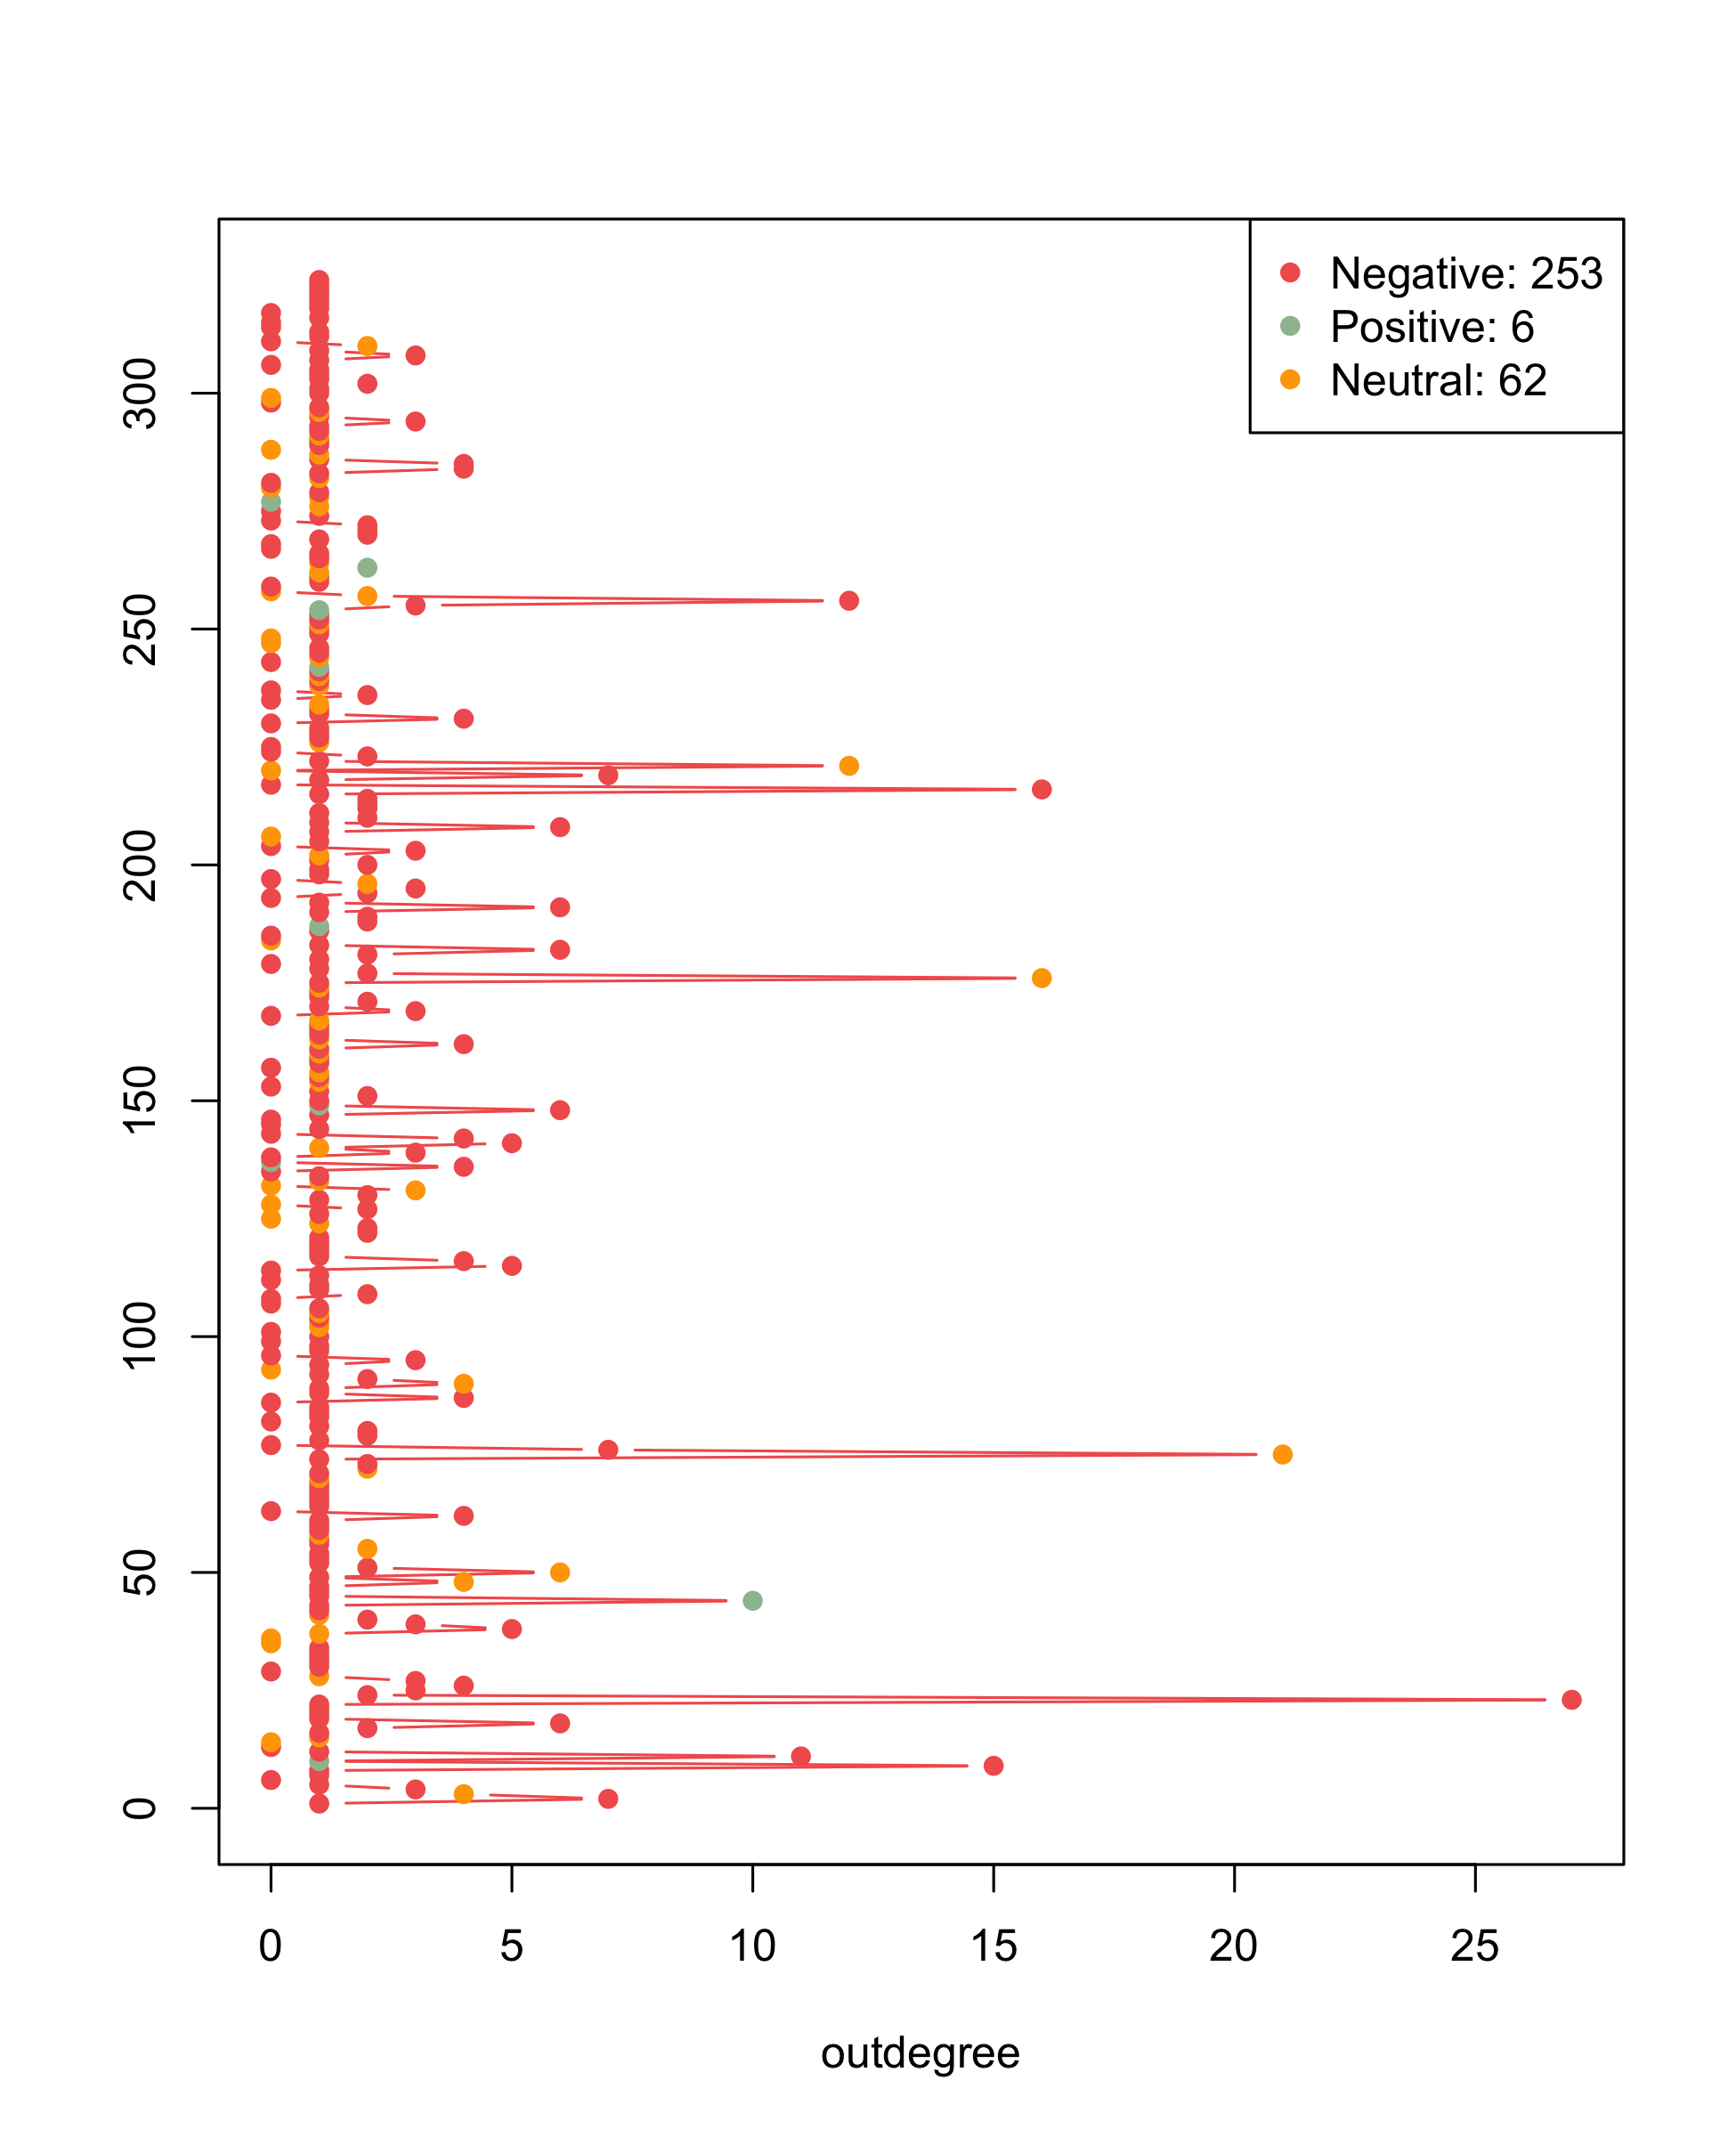
\includegraphics{SNA4DS_Report_files/figure-latex/outdegree-plot-1} \caption{The outdegree plotted for each node in the network}\label{fig:outdegree-plot}
\end{figure}

\section{\texorpdfstring{ERGM Results\\
}{ERGM Results }}\label{ergm-results}

We display the results of the different models we ran as well as the diagnostics for model 5.\\


\begin{Shaded}
\begin{Highlighting}[]
\NormalTok{texreg}\SpecialCharTok{::}\FunctionTok{plotreg}\NormalTok{(models)}
\end{Highlighting}
\end{Shaded}

\begin{figure}[H]
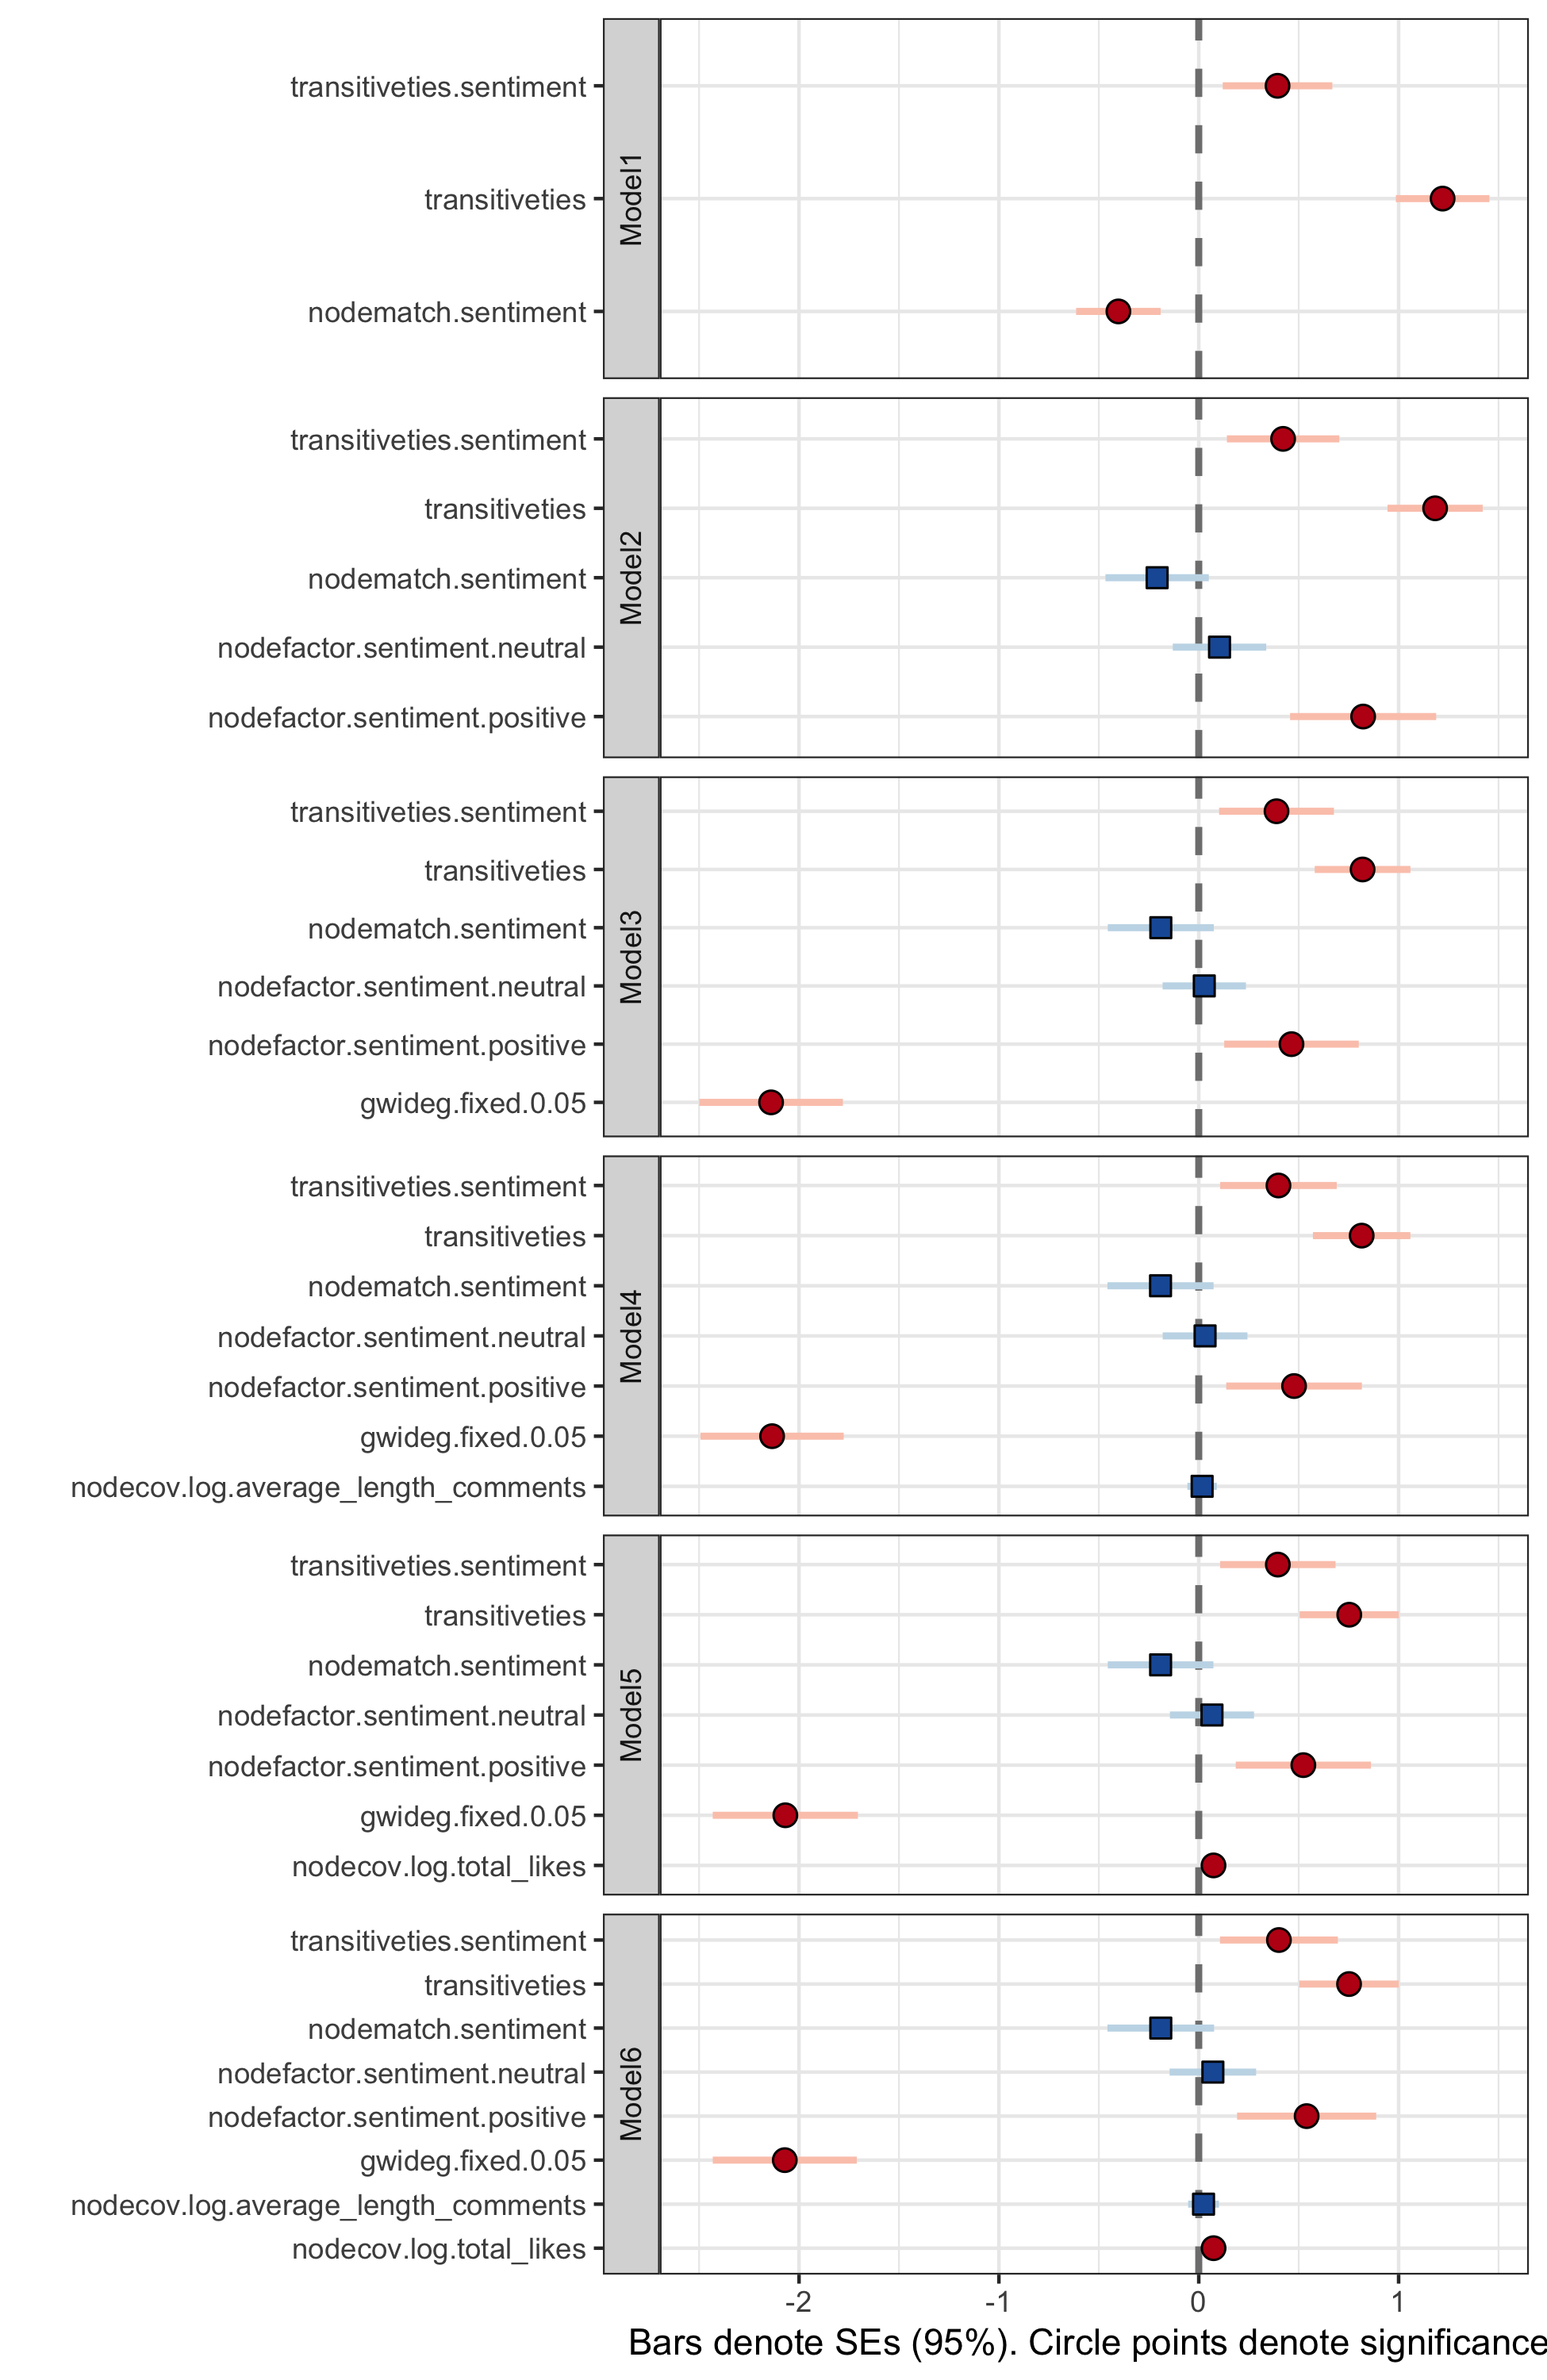
\includegraphics{SNA4DS_Report_files/figure-latex/ergm-results-plot-1} \caption{ }\label{fig:ergm-results-plot}
\end{figure}
\newpage

\subsection{\texorpdfstring{Model Diagnostics of model 5\\
}{Model Diagnostics of model 5 }}\label{model-diagnostics-of-model-5}



\begin{Shaded}
\begin{Highlighting}[]
\CommentTok{\# Plotting MCMC diagnostic}
\NormalTok{model\_5 }\OtherTok{\textless{}{-}}\NormalTok{ models}\SpecialCharTok{$}\NormalTok{model\_5}
\FunctionTok{par}\NormalTok{(}\AttributeTok{mai=}\FunctionTok{c}\NormalTok{(.}\DecValTok{6}\NormalTok{,}\FloatTok{0.3}\NormalTok{,.}\DecValTok{4}\NormalTok{,}\FloatTok{0.3}\NormalTok{), }\AttributeTok{omi=}\FunctionTok{c}\NormalTok{(.}\DecValTok{1}\NormalTok{,.}\DecValTok{1}\NormalTok{,.}\DecValTok{1}\NormalTok{,.}\DecValTok{1}\NormalTok{)) }\CommentTok{\# setting margins due to error}

\NormalTok{ergm}\SpecialCharTok{::}\FunctionTok{mcmc.diagnostics}\NormalTok{(}
\NormalTok{  model\_5,}
  \AttributeTok{which =} \FunctionTok{c}\NormalTok{(}\StringTok{"plots"}\NormalTok{)}
\NormalTok{  )}
\end{Highlighting}
\end{Shaded}

\begin{figure}[H]

{\centering 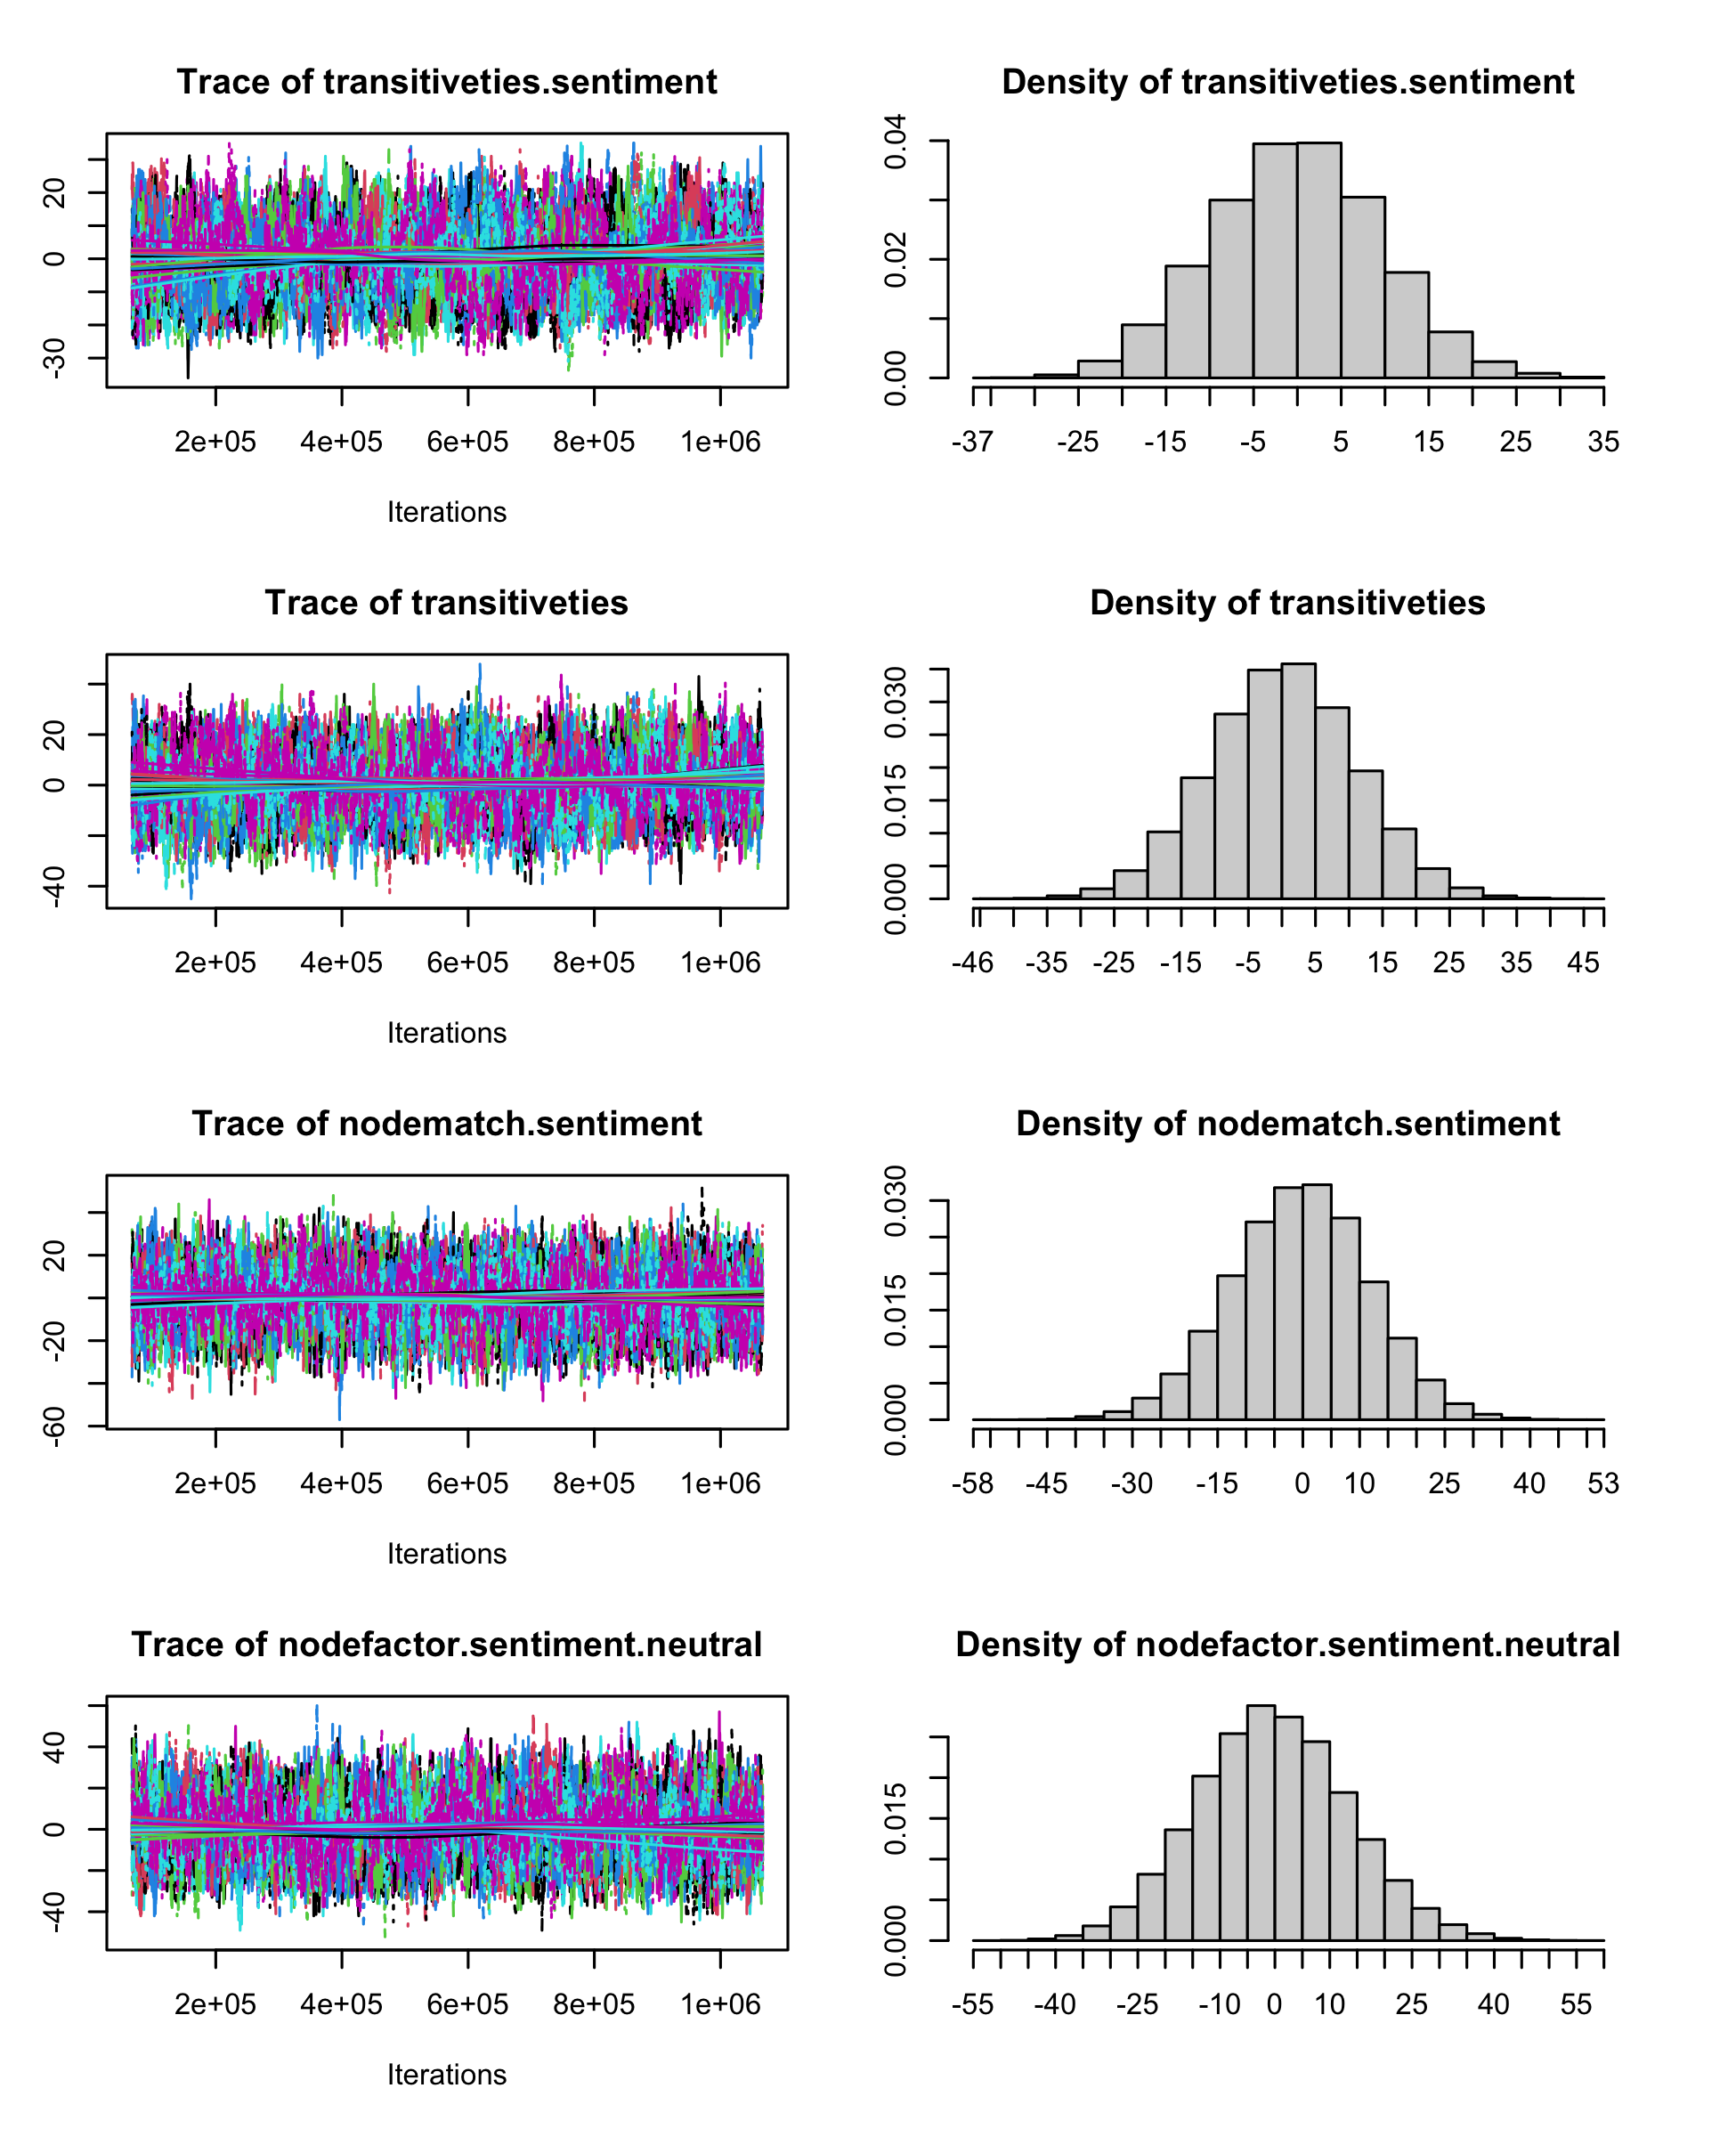
\includegraphics{SNA4DS_Report_files/figure-latex/mcmc-diagnostics-1} 

}

\caption{The MCMC diagnostics for model 5.}\label{fig:mcmc-diagnostics-1}
\end{figure}
\begin{figure}[H]

{\centering 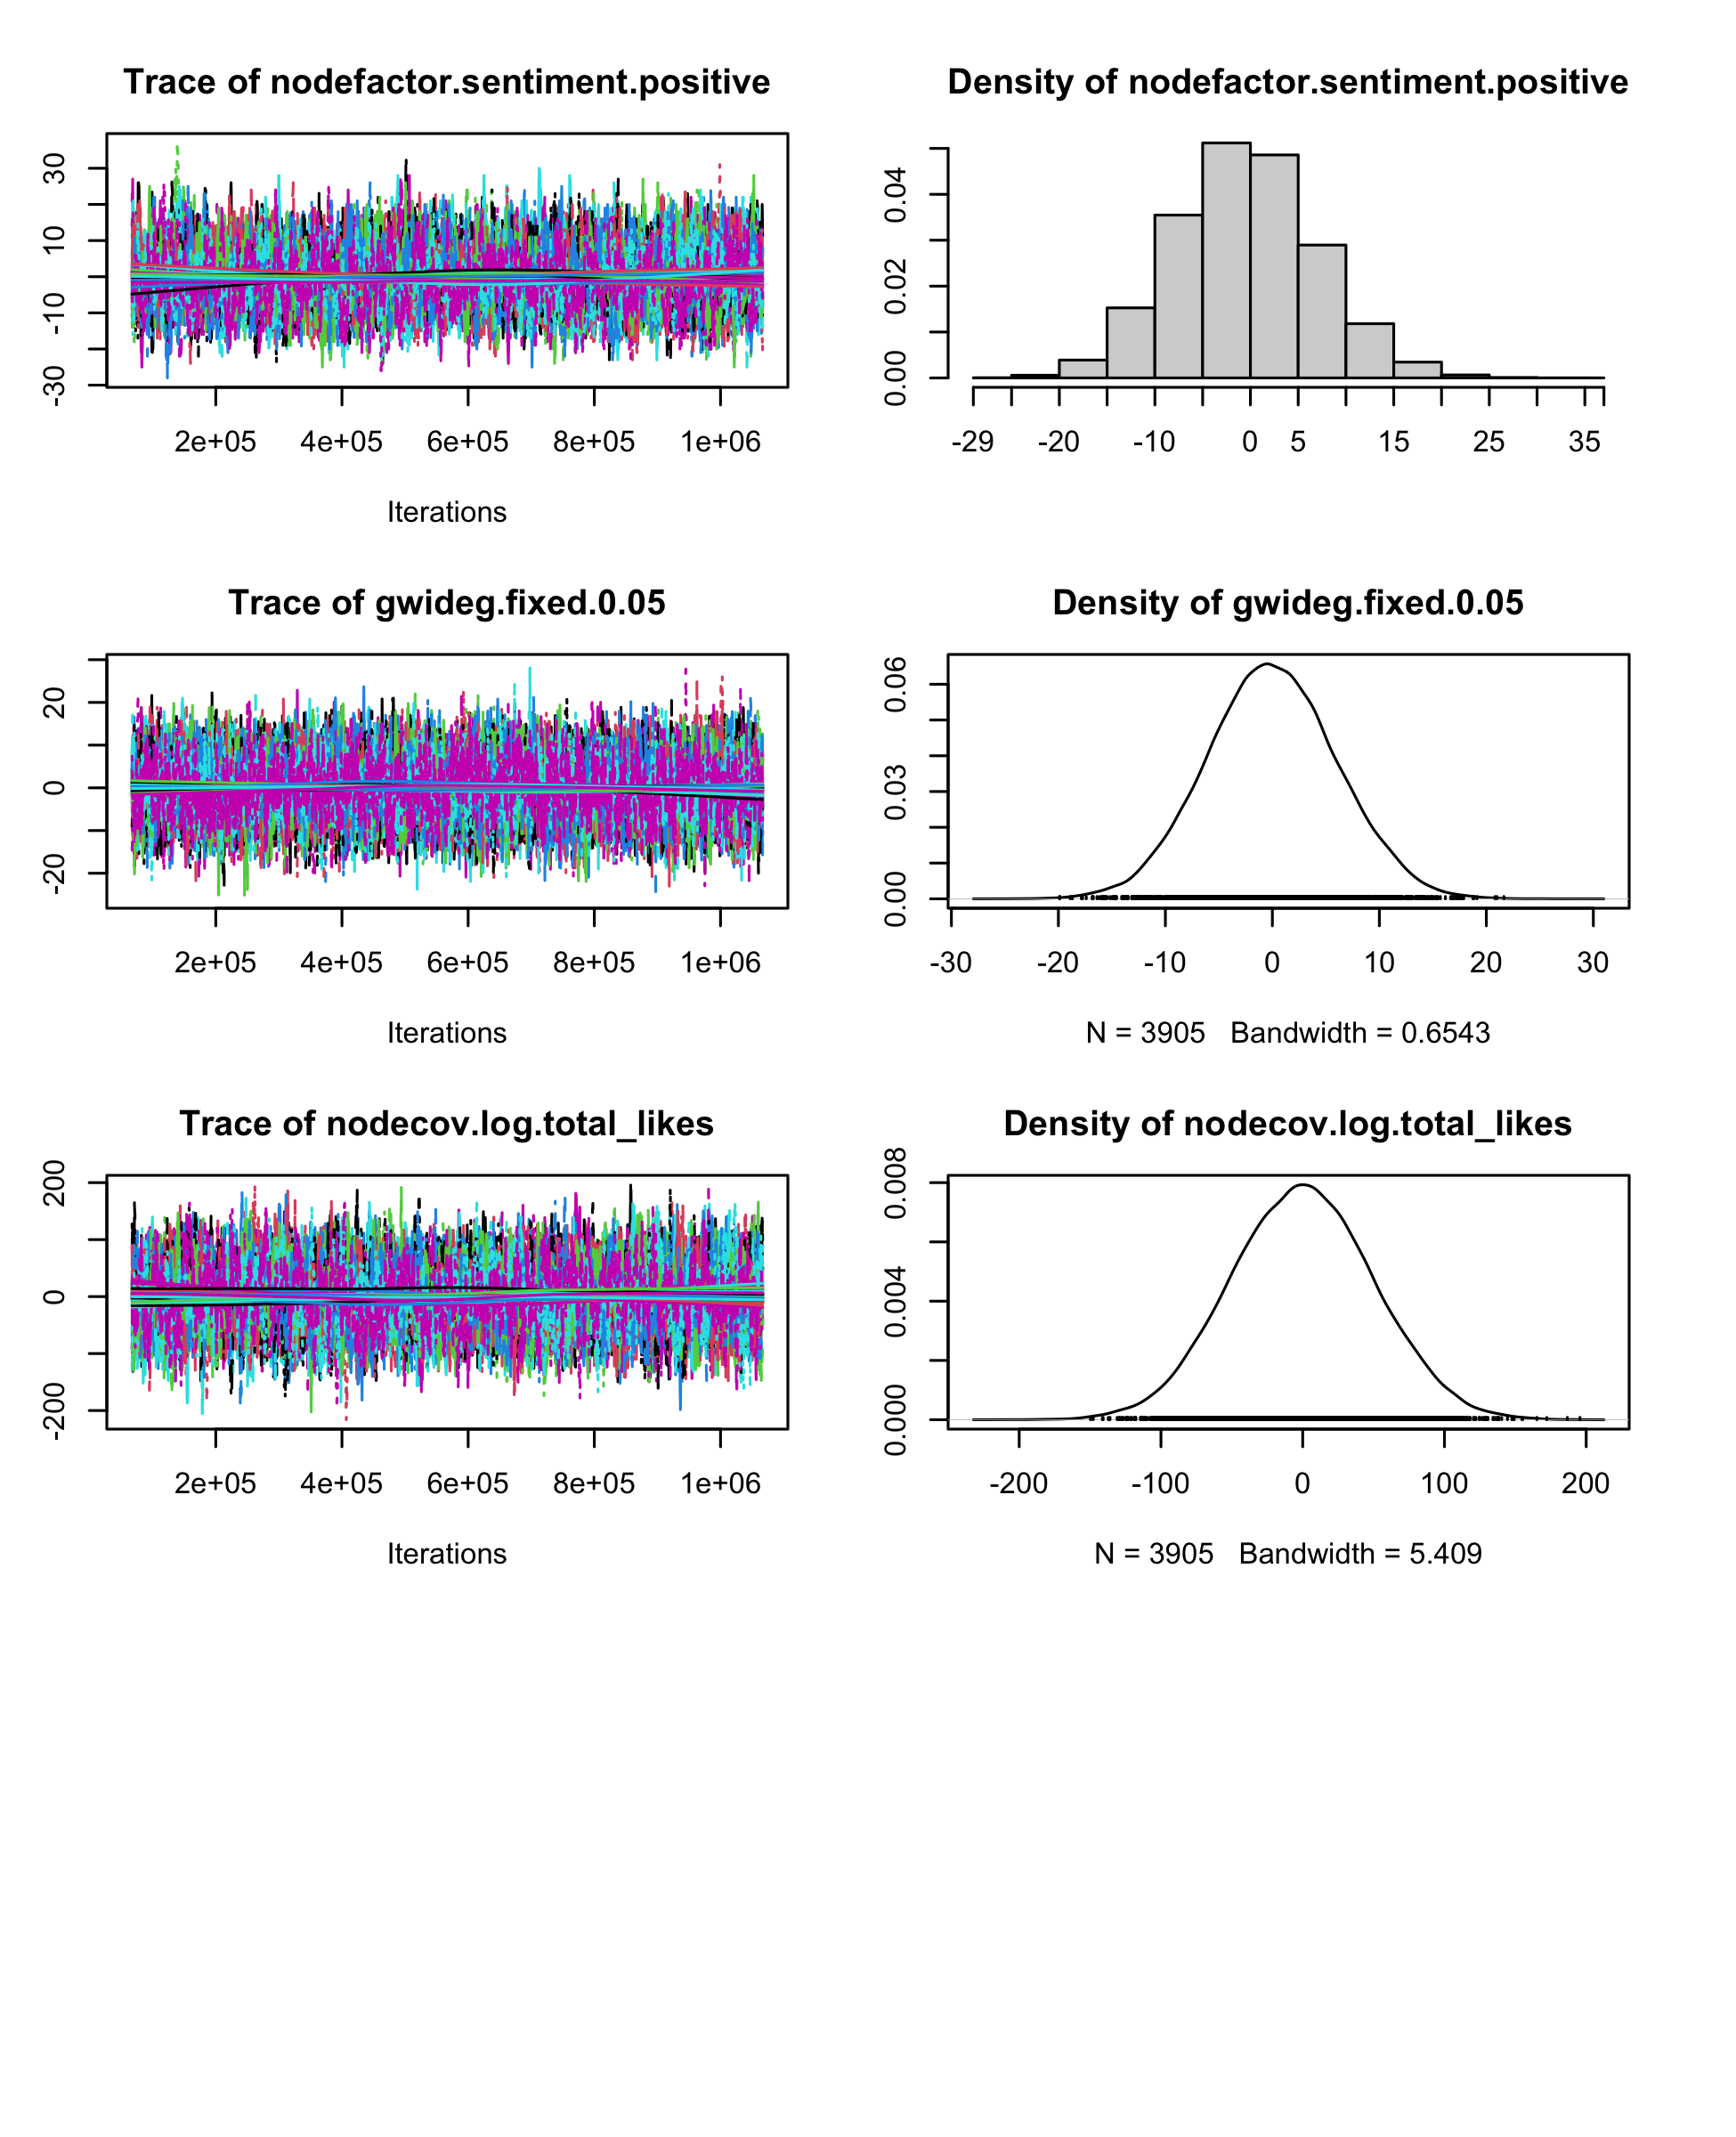
\includegraphics{SNA4DS_Report_files/figure-latex/mcmc-diagnostics-2} 

}

\caption{The MCMC diagnostics for model 5.}\label{fig:mcmc-diagnostics-2}
\end{figure}

Note: MCMC diagnostics shown here are from the last round of
simulation, prior to computation of final parameter estimates.
Because the final estimates are refinements of those used for this
simulation run, these diagnostics may understate model performance.
To directly assess the performance of the final model on in-model
statistics, please use the GOF command: gof(ergmFitObject,
GOF=\textasciitilde model).
\newpage

\subsection{\texorpdfstring{Goodness of Fit of model 5\\
}{Goodness of Fit of model 5 }}\label{goodness-of-fit-of-model-5}



\begin{figure}[H]
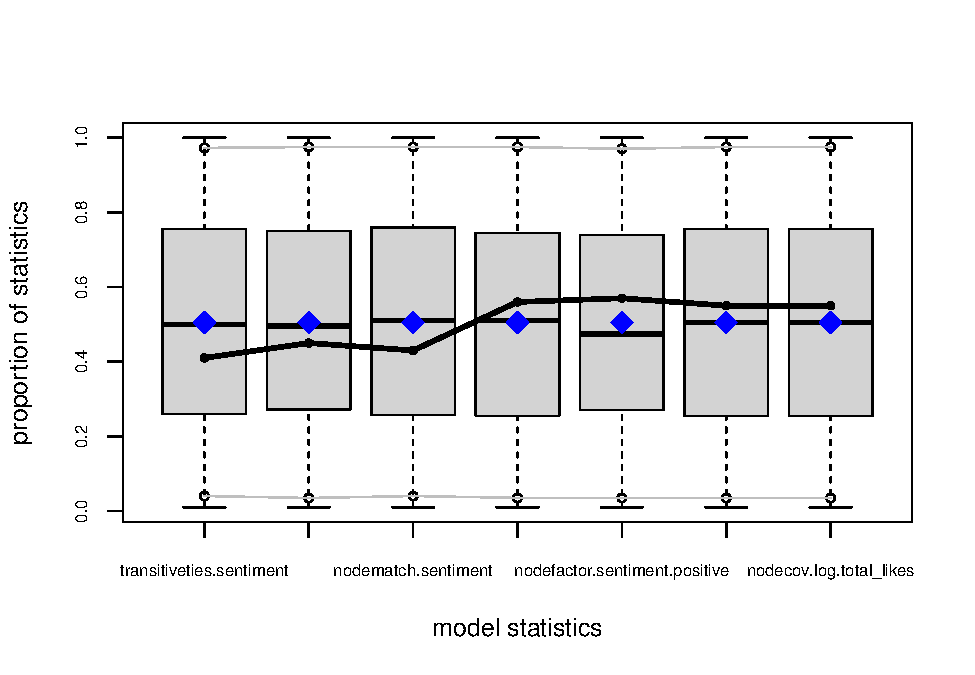
\includegraphics{SNA4DS_Report_files/figure-latex/gof-model5-1} \caption{The plot below shows the Goodness of Fit statistics for model 5}\label{fig:gof-model5-1}
\end{figure}
\begin{figure}[H]
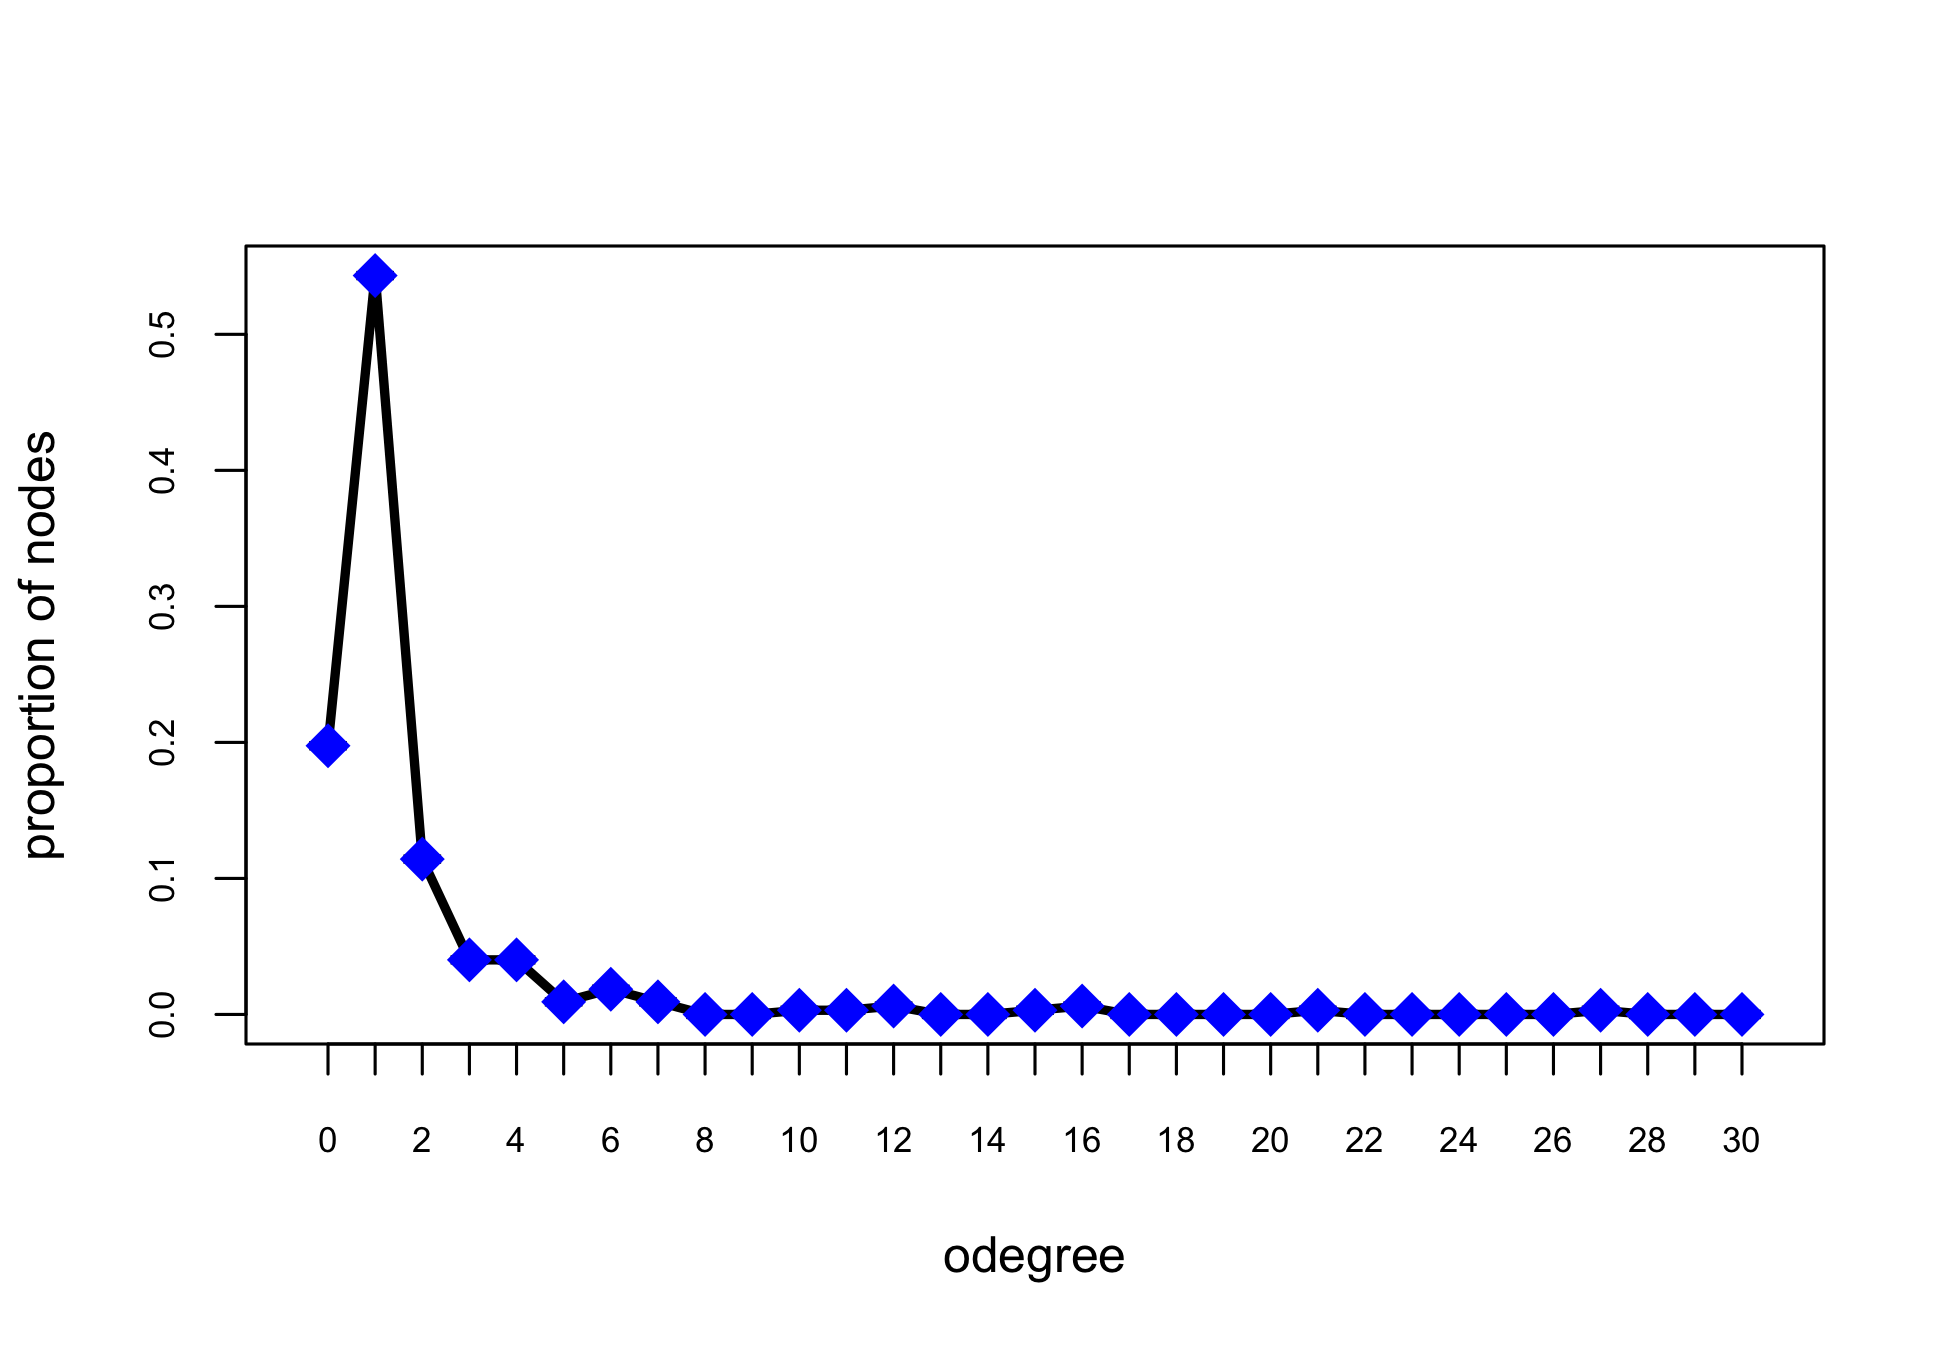
\includegraphics{SNA4DS_Report_files/figure-latex/gof-model5-2} \caption{The plot below shows the Goodness of Fit statistics for model 5}\label{fig:gof-model5-2}
\end{figure}
\begin{figure}[H]
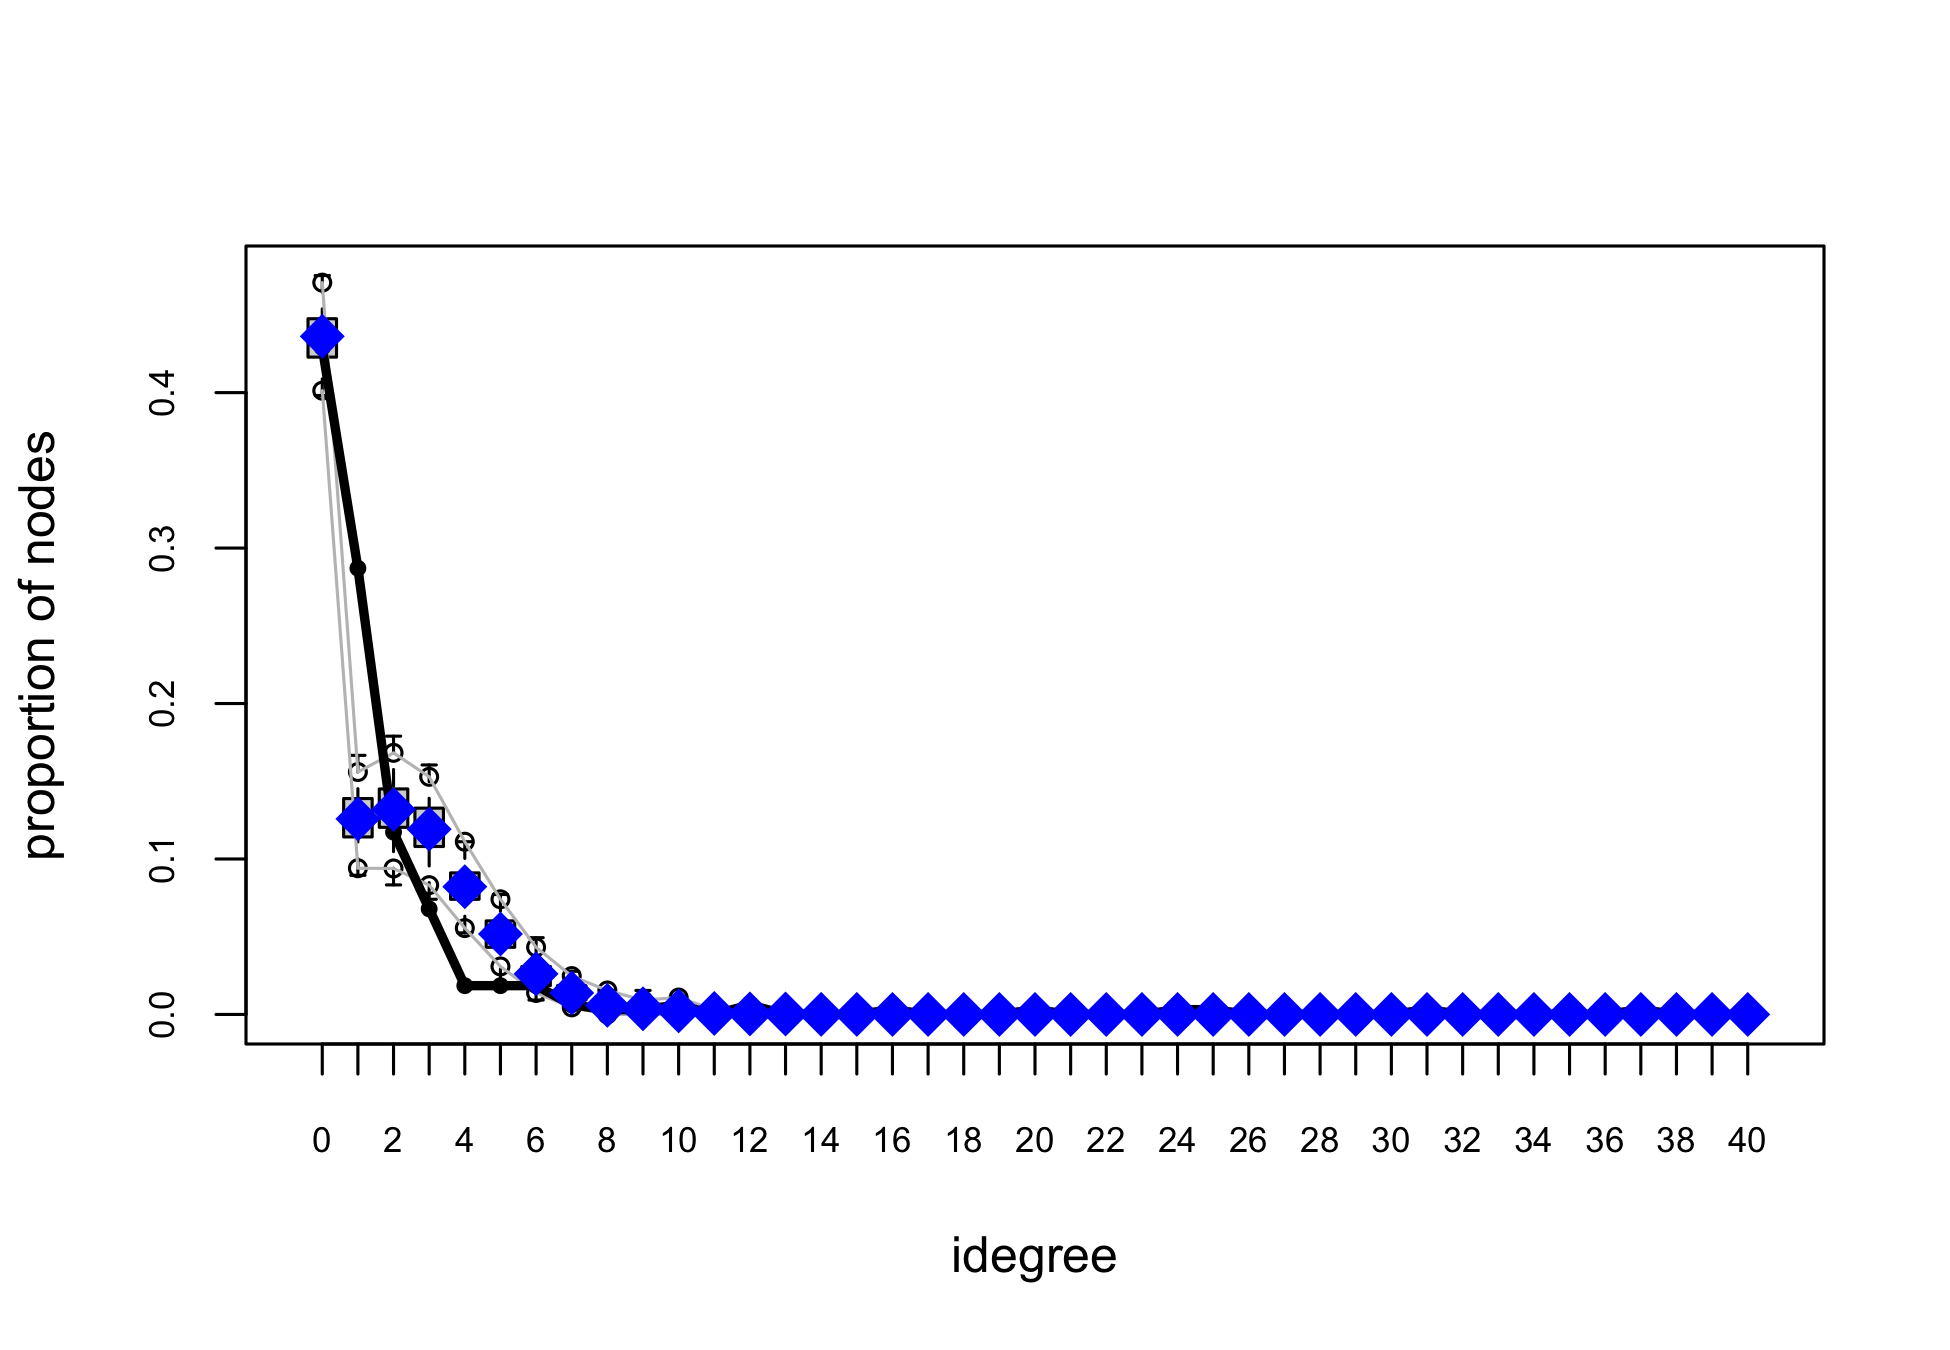
\includegraphics{SNA4DS_Report_files/figure-latex/gof-model5-3} \caption{The plot below shows the Goodness of Fit statistics for model 5}\label{fig:gof-model5-3}
\end{figure}
\begin{figure}[H]
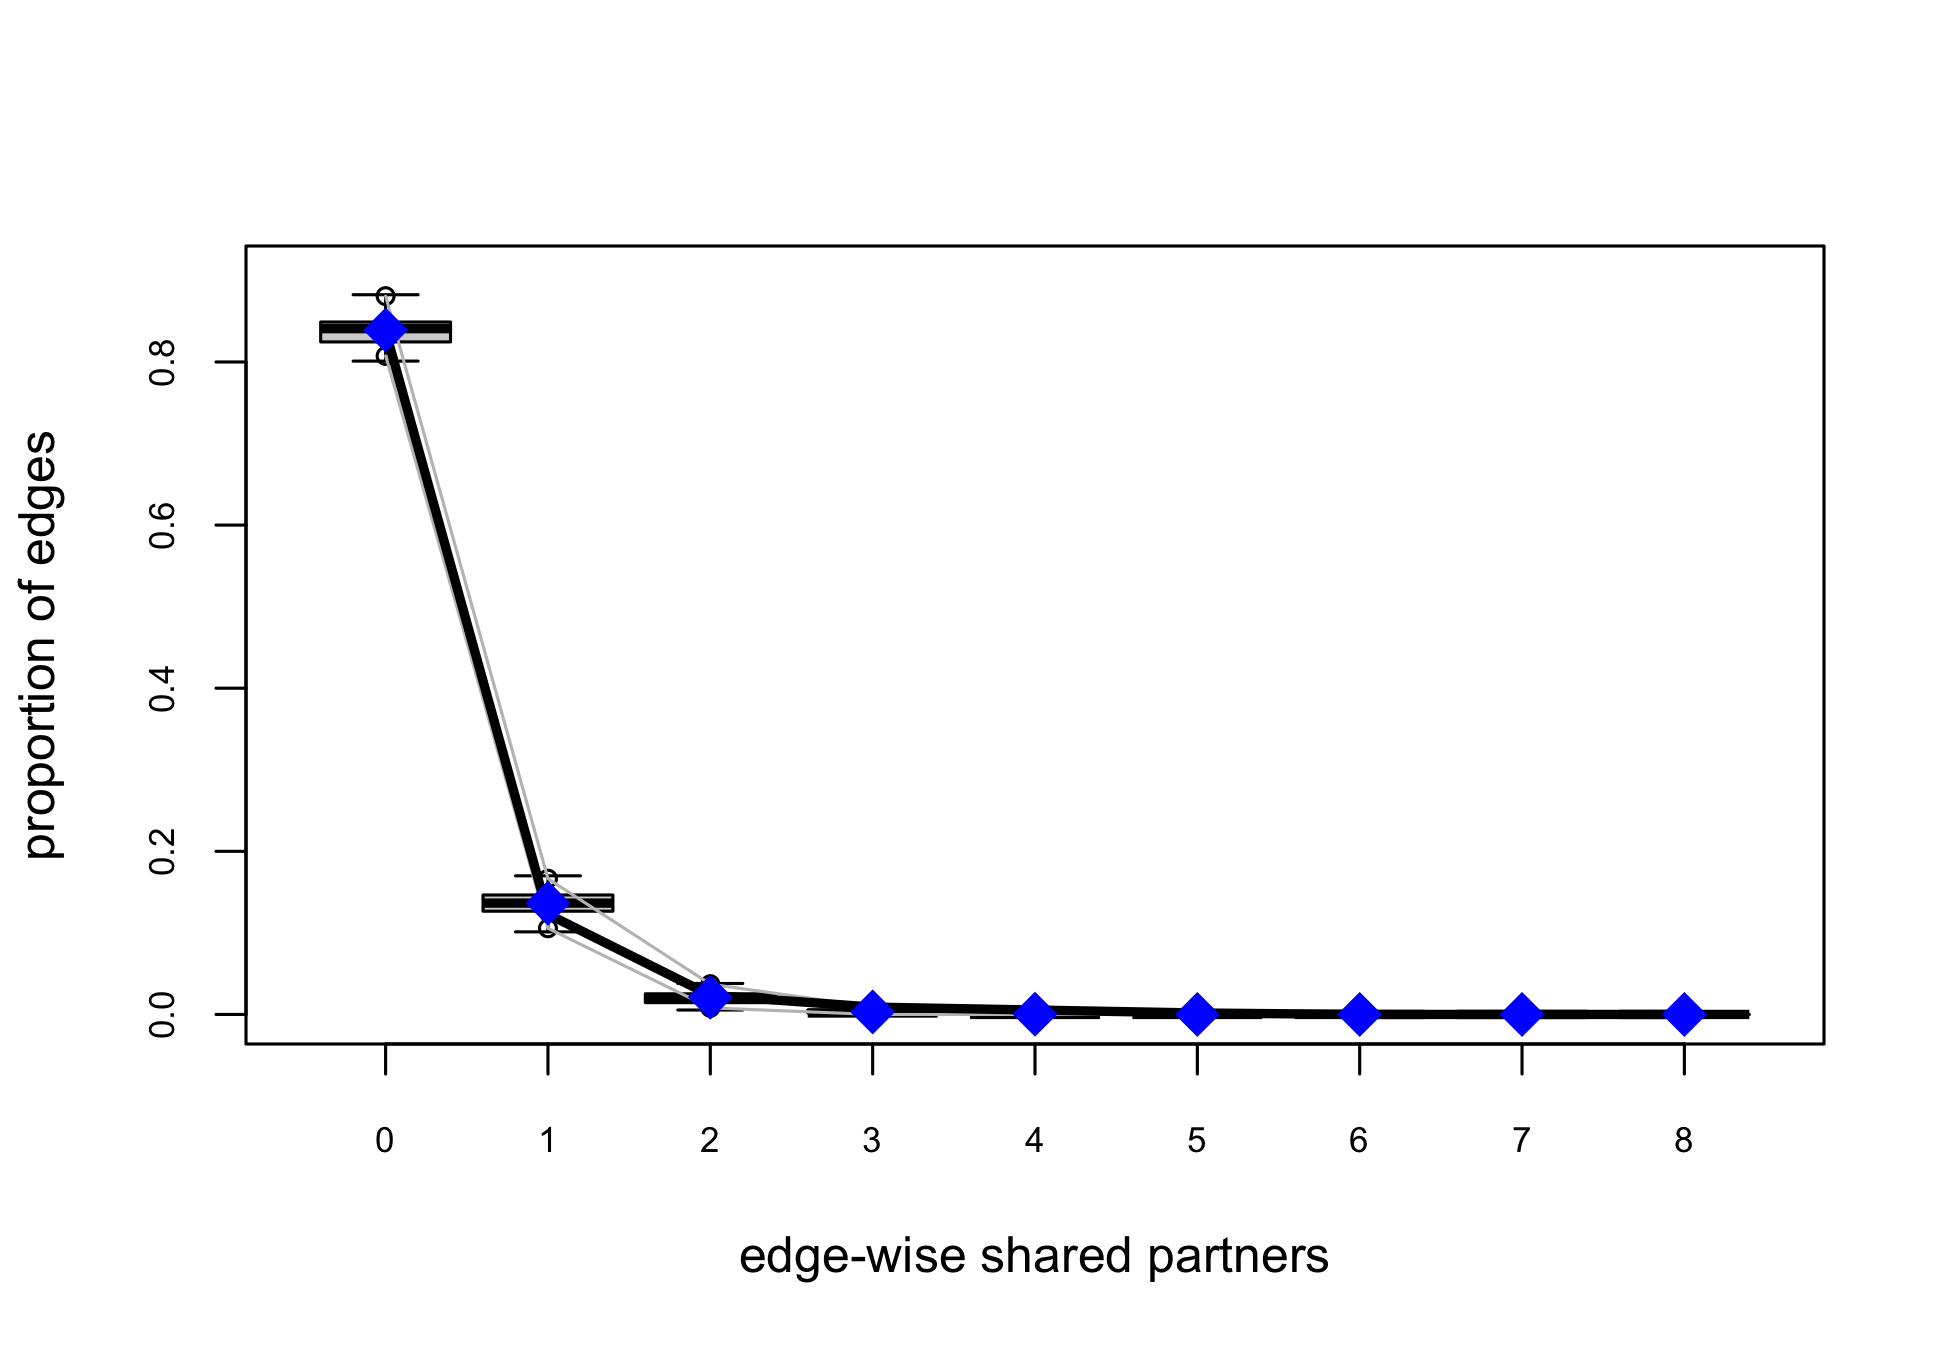
\includegraphics{SNA4DS_Report_files/figure-latex/gof-model5-4} \caption{The plot below shows the Goodness of Fit statistics for model 5}\label{fig:gof-model5-4}
\end{figure}
\begin{figure}[H]
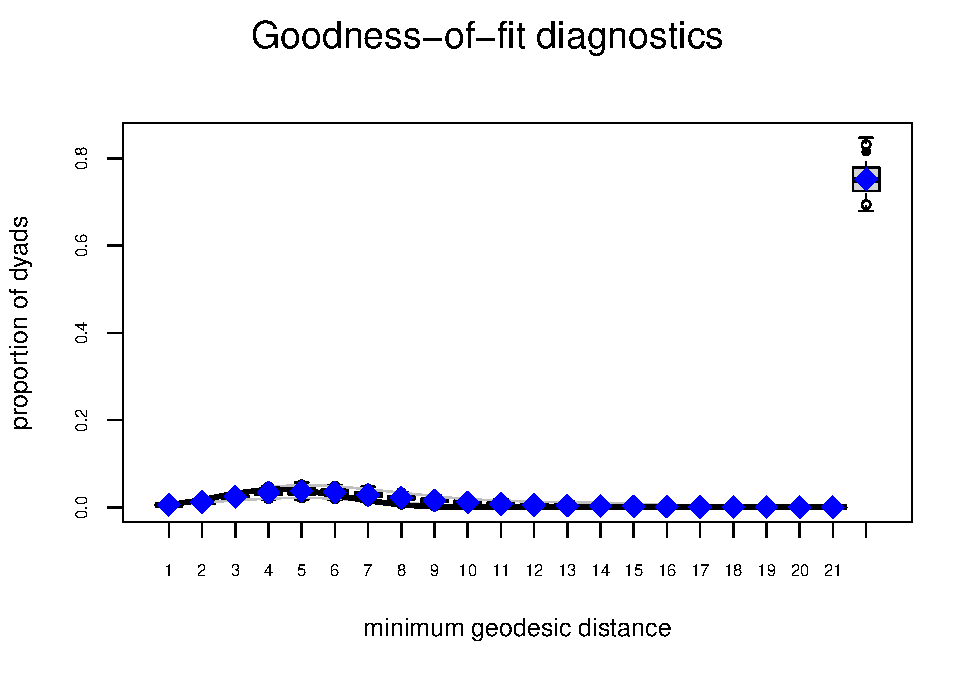
\includegraphics{SNA4DS_Report_files/figure-latex/gof-model5-5} \caption{The plot below shows the Goodness of Fit statistics for model 5}\label{fig:gof-model5-5}
\end{figure}


\end{document}
